\subsection{Values}

\begin{frame}
	\large
	{\Large Values of any transport system}
	\begin{enumerate}
		\item Safety
		\item Generate wealth
		\item Speed
	\end{enumerate}
	\vspace{1em}
	{\Large Bratislava transit plan}
	\begin{enumerate}
		\item Trams
		\item Trains
		\item Cars
		\item \textbf{NO} metro >:( - doesn't make sense financially
	\end{enumerate}
\end{frame}

\subsection{What we have learned about building transport}

\begin{frame}
	\frametitle{Transportation}
	\framesubtitle{What is the difference between a street, stroad and a road?}
	
	\small
	\begin{columns}
		\begin{column}{0.32\textwidth}
			\centering
			{\Large Street\\[0.5em]}
			\includegraphics[width=\textwidth]{obchodna}

			\only<2->{\begin{enumerate}
				\item Generates wealth
				\item Is the destination
				\item \underline{Complex}
			\end{enumerate}}
		\end{column}
		\begin{column}{0.32\textwidth}
			\centering
			{\Large Road\\[.5em]}
			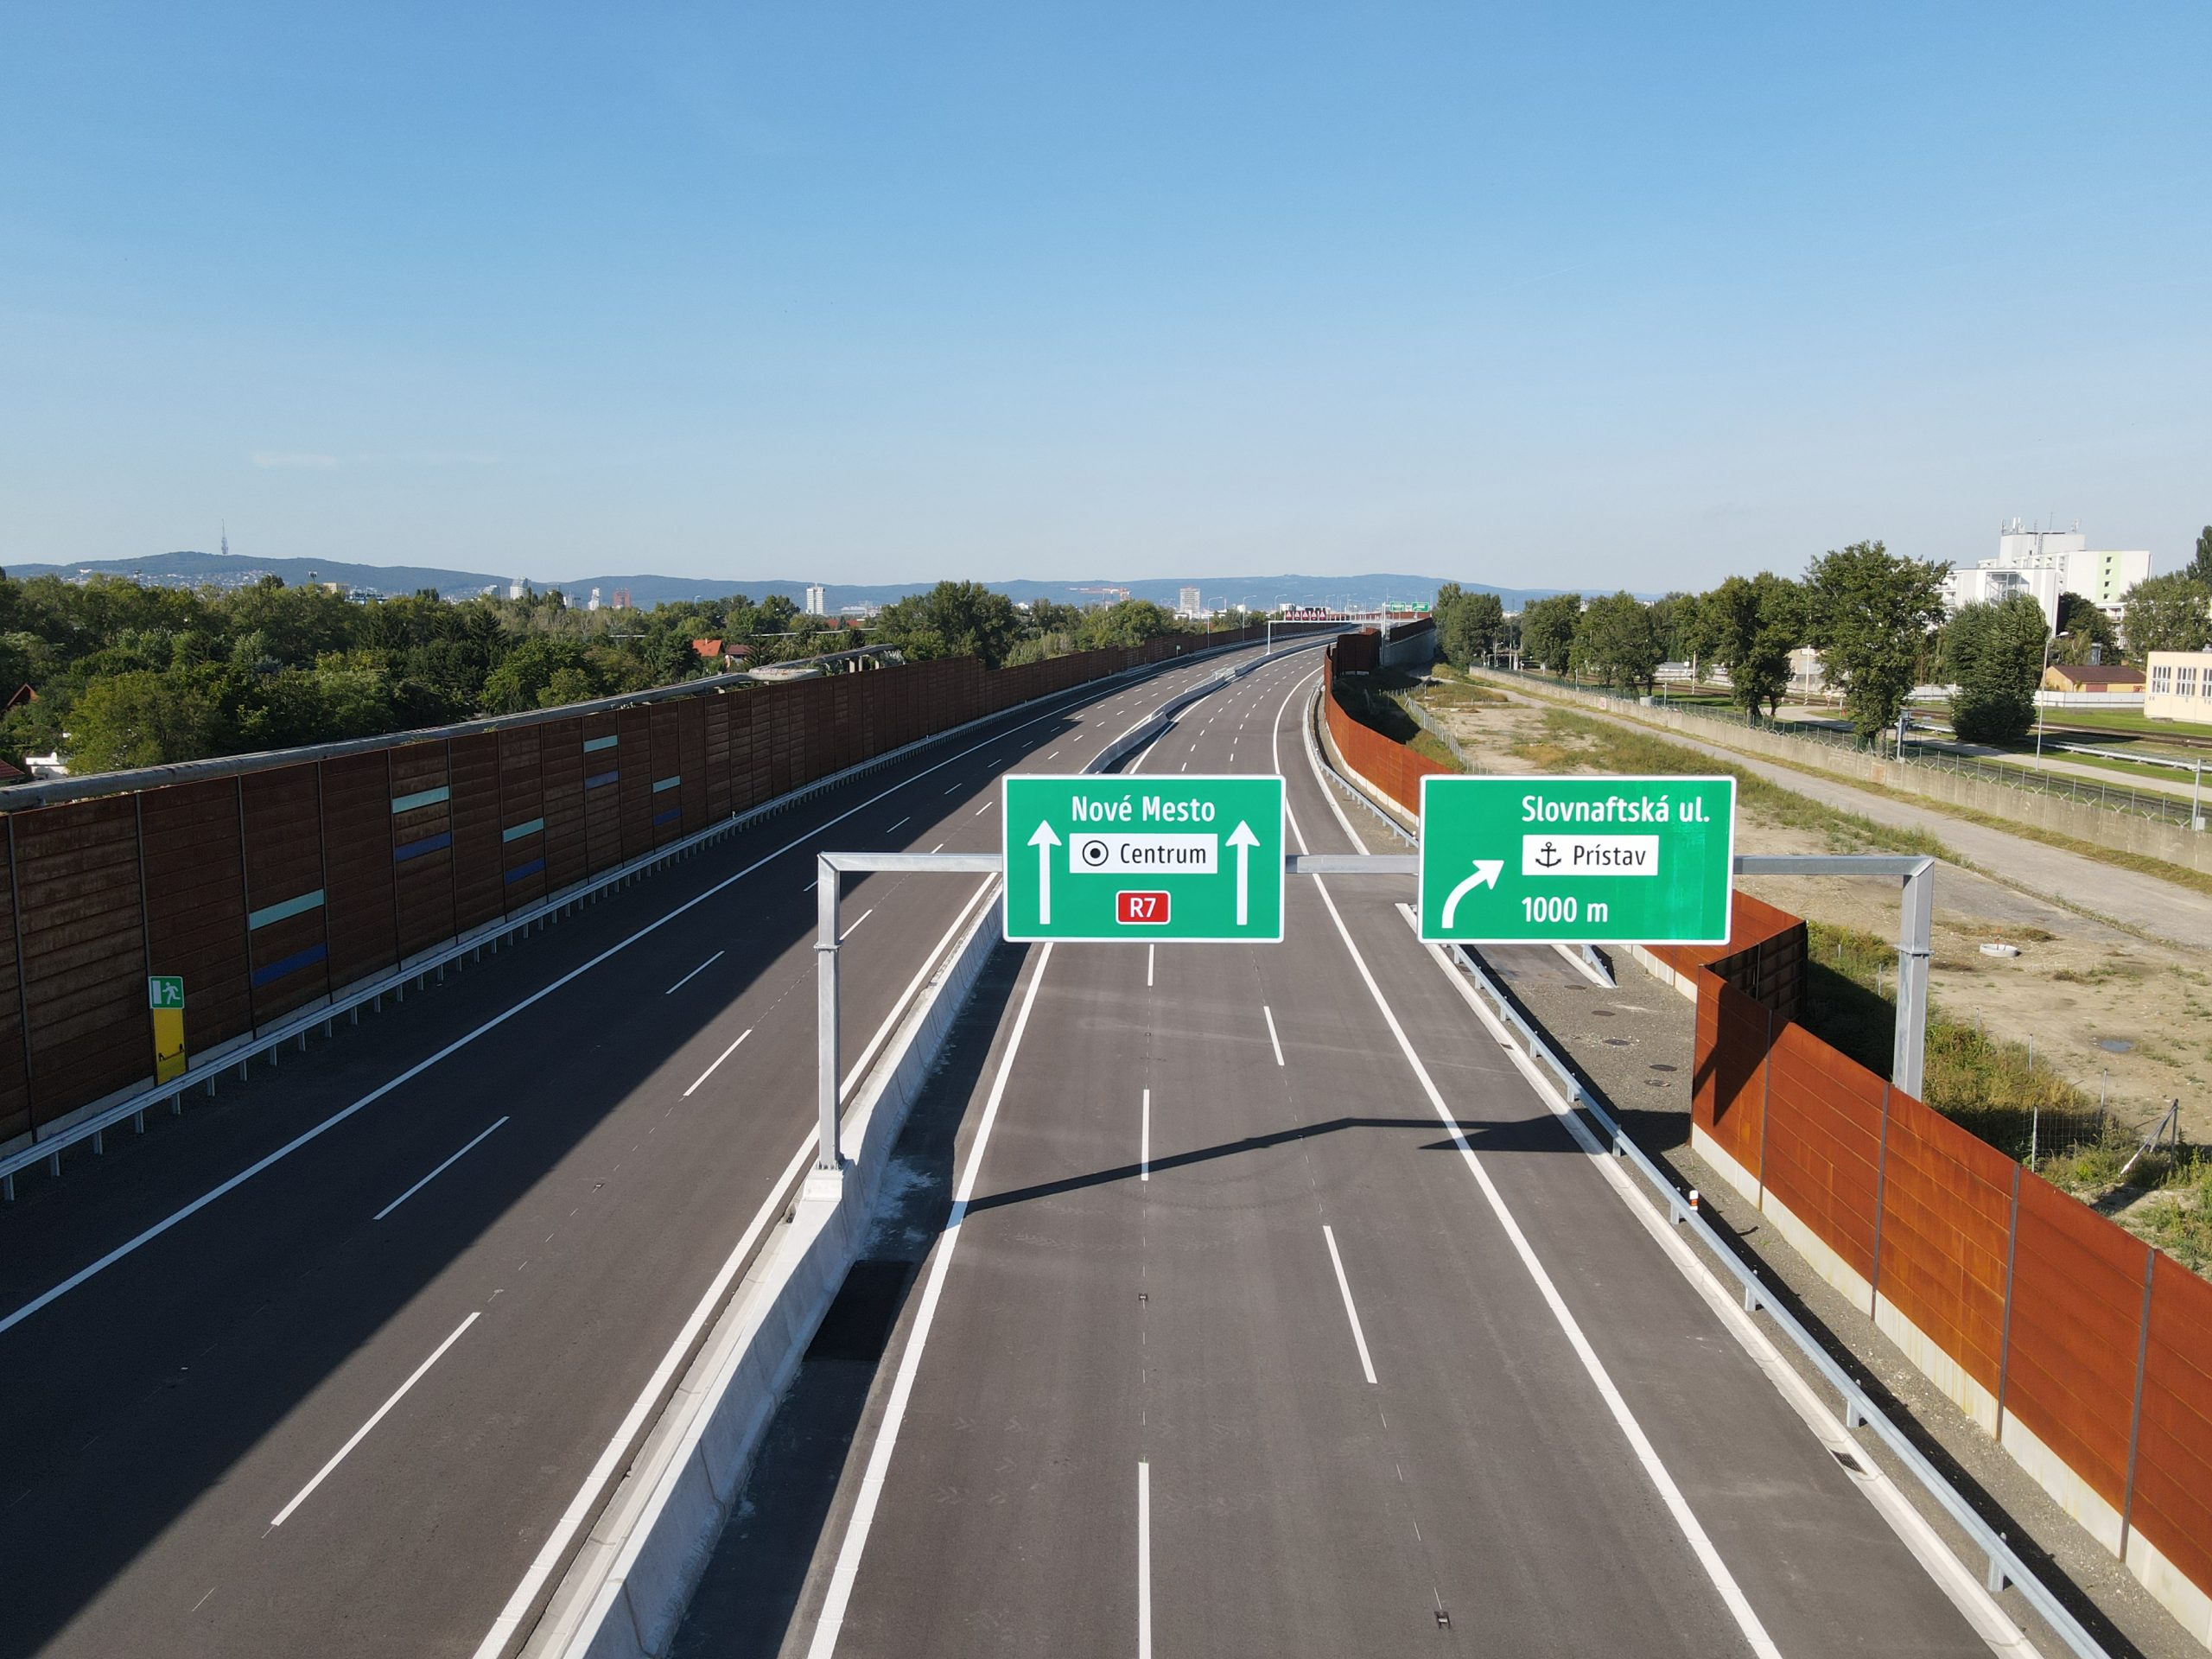
\includegraphics[width=\textwidth]{r7}						

			\only<3->{\begin{enumerate}
				\item Suited for cars only
				\item Connect destinations
				\item \underline{Simple}
			\end{enumerate}}
		\end{column}
		\begin{column}{0.32\textwidth}
			\centering
			{\Large Stroad\\[.5em]}
			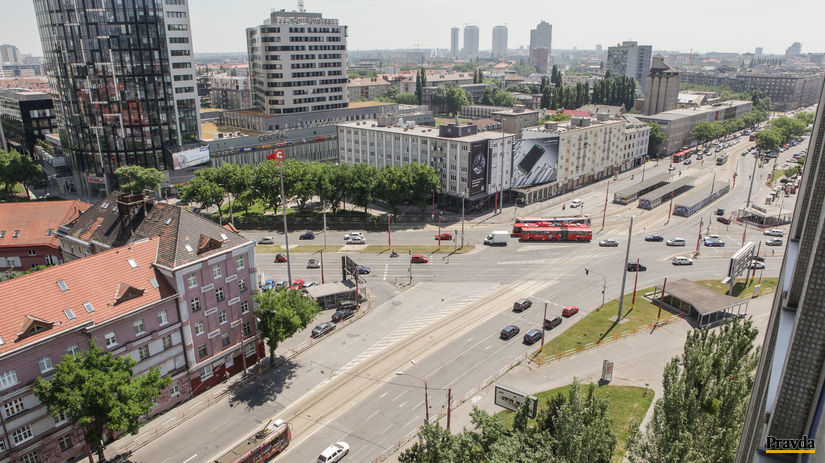
\includegraphics[width=\textwidth]{trnavske}

			\only<4->{\begin{enumerate}
				\item Tries to make cars fast, only to stop them on a traffic light
				\item Dangerous
				\item Wastes land
				\item \underline{Stupid}
			\end{enumerate}}
		\end{column}
	\end{columns}
\end{frame}

\section{The present}

\subsection{The good}

\begin{frame}
	\frametitle{The Double Plus Good}
	\centering
	\only<1>{
	\framesubtitle{Dubravka}
	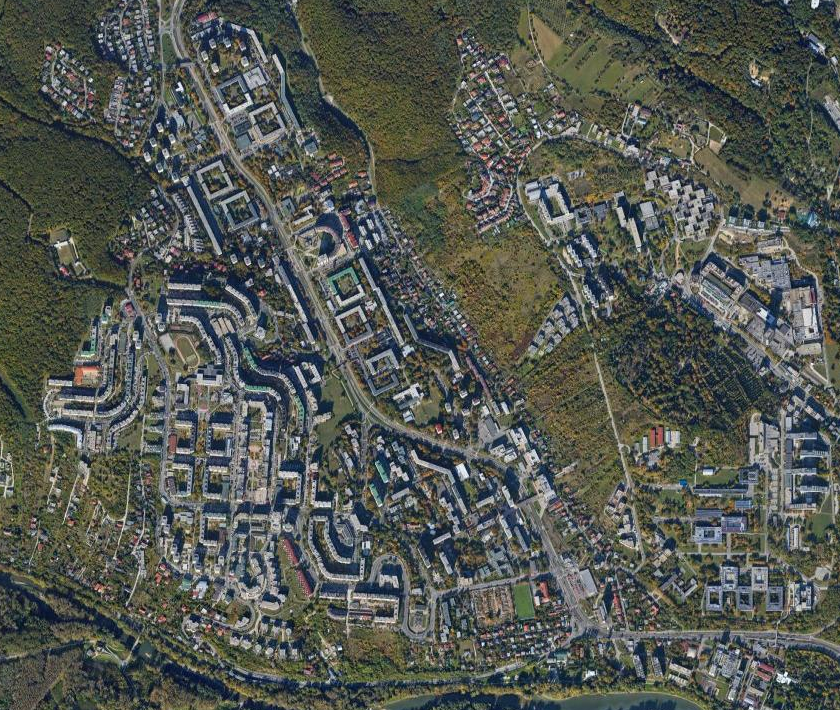
\includegraphics[height=.4\textheight]{dubravka}\\
	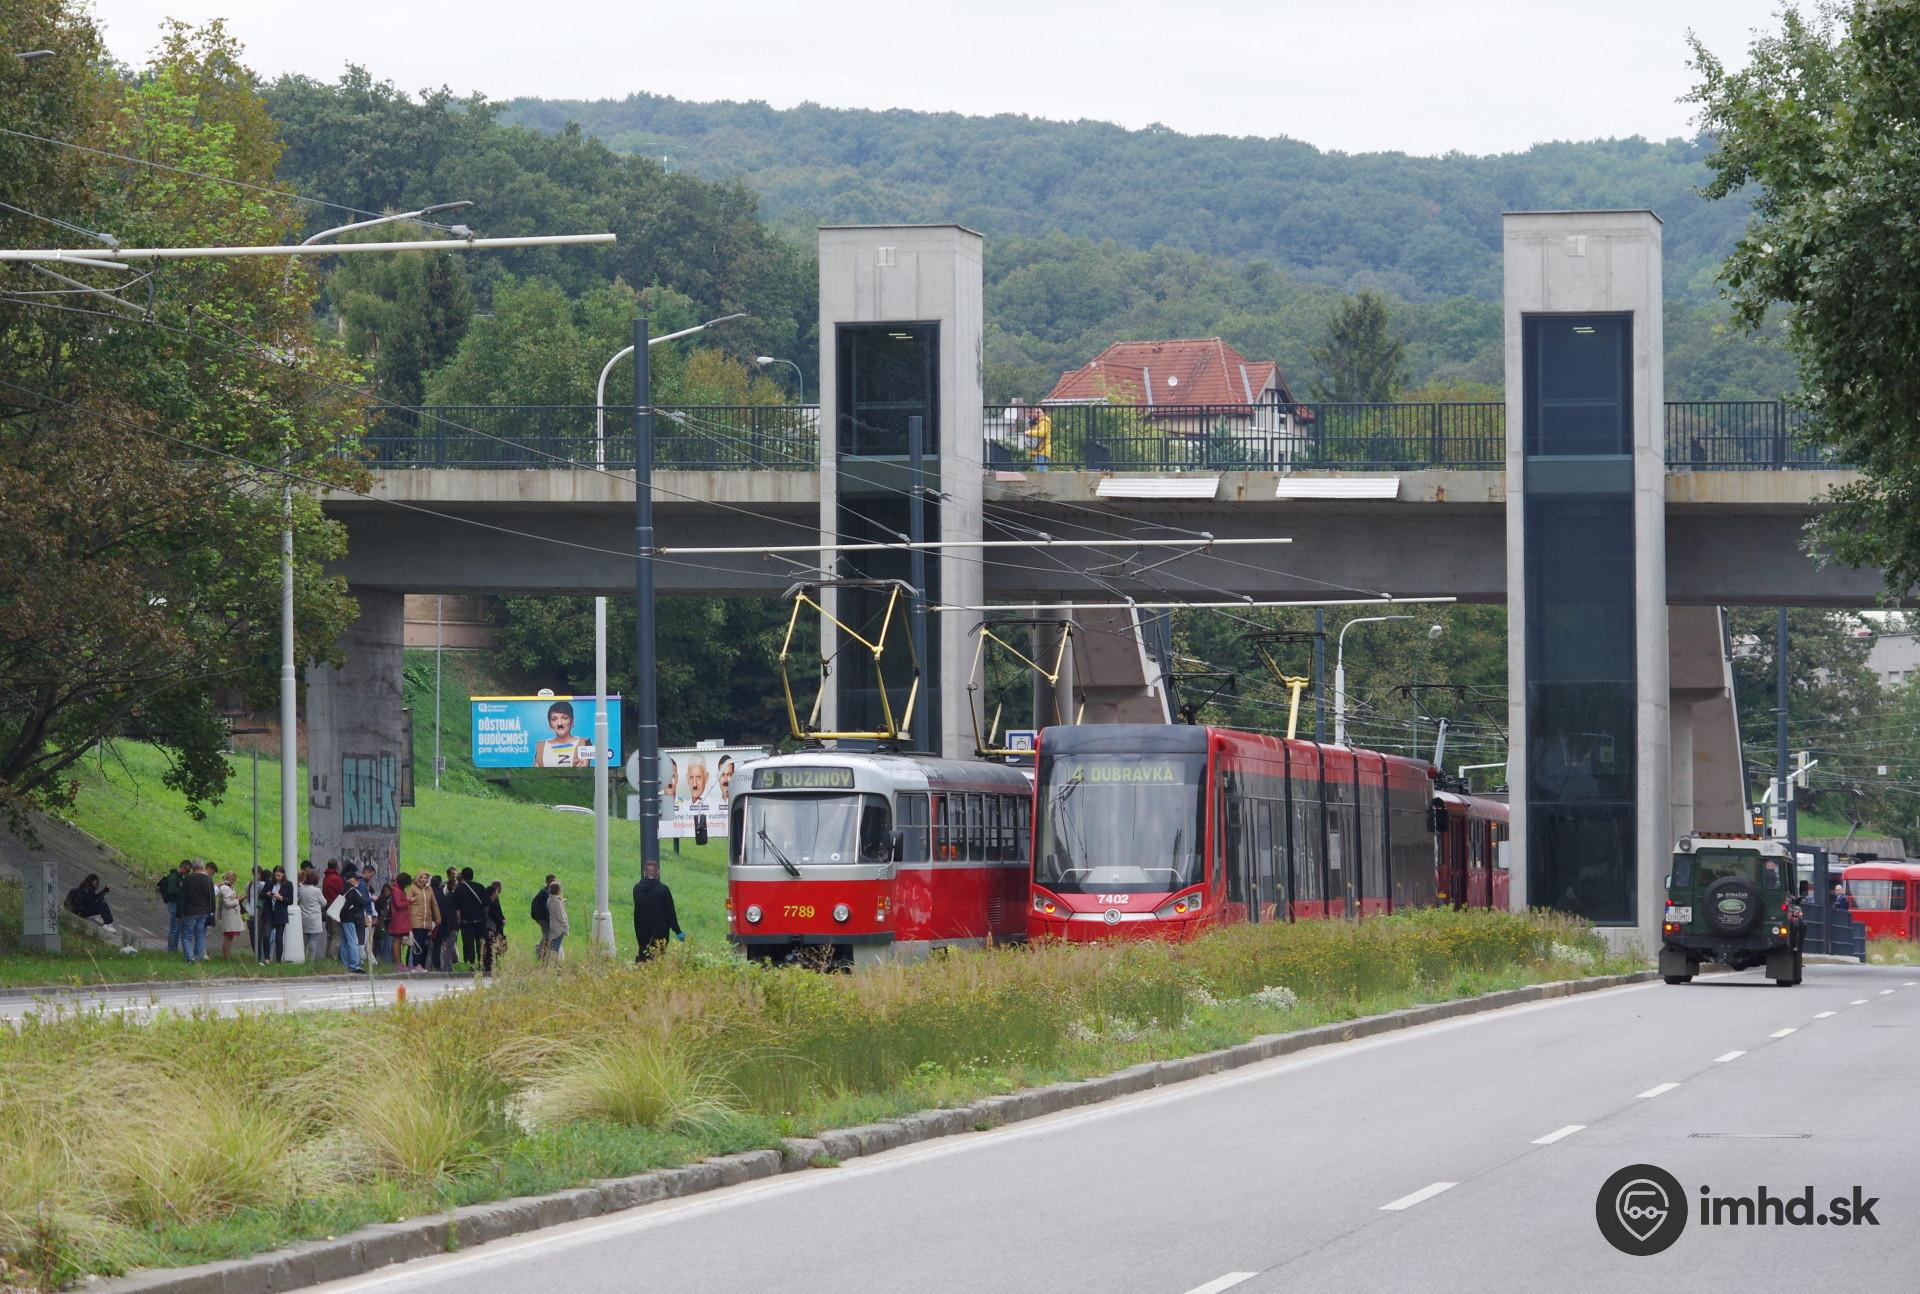
\includegraphics[height=.4\textheight]{dubravka-mlynska-dolina}}
	\only<2>{
	\framesubtitle{Ružinov}
	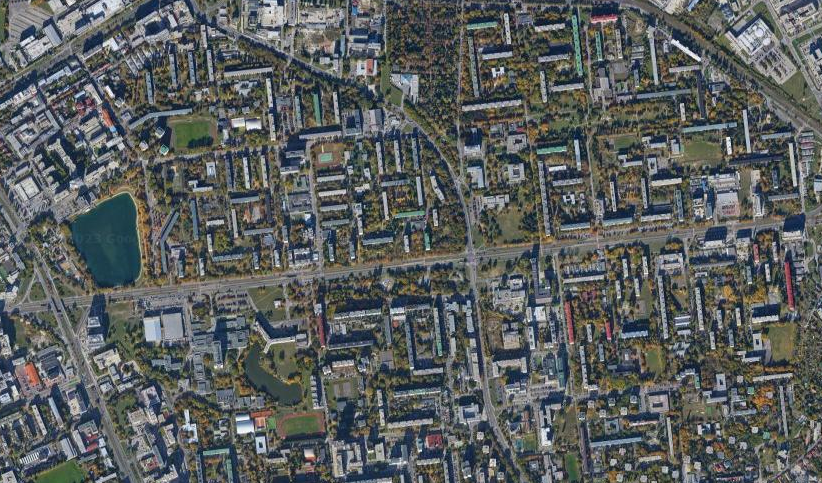
\includegraphics[height=.4\textheight]{ruzinov}\\
	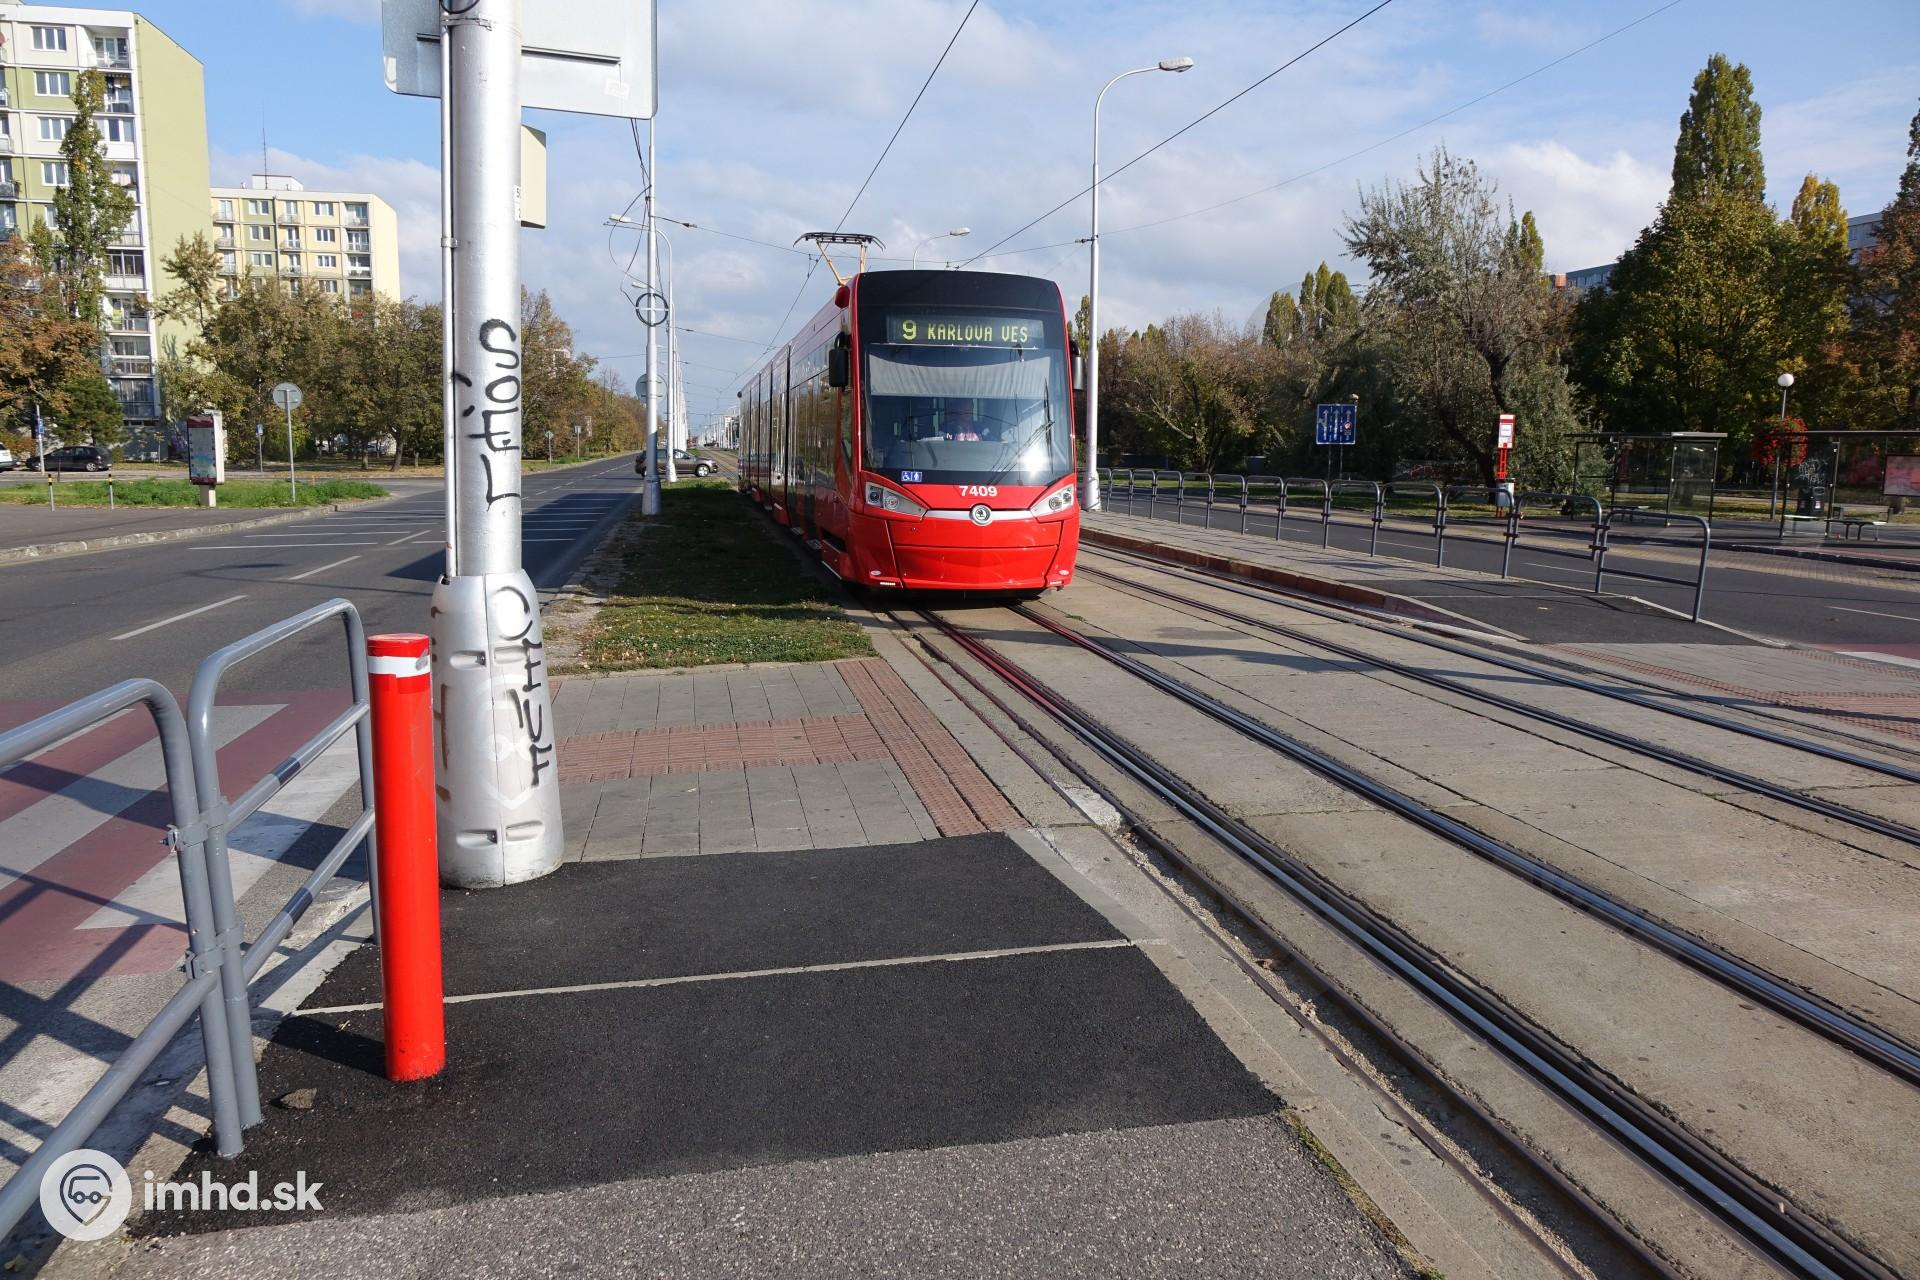
\includegraphics[height=.4\textheight]{ruzinov-herlianska}}
\end{frame}

\subsection{The Bad}

\begin{frame}
	\centering
	\frametitle{Stroads}
	\only<1>{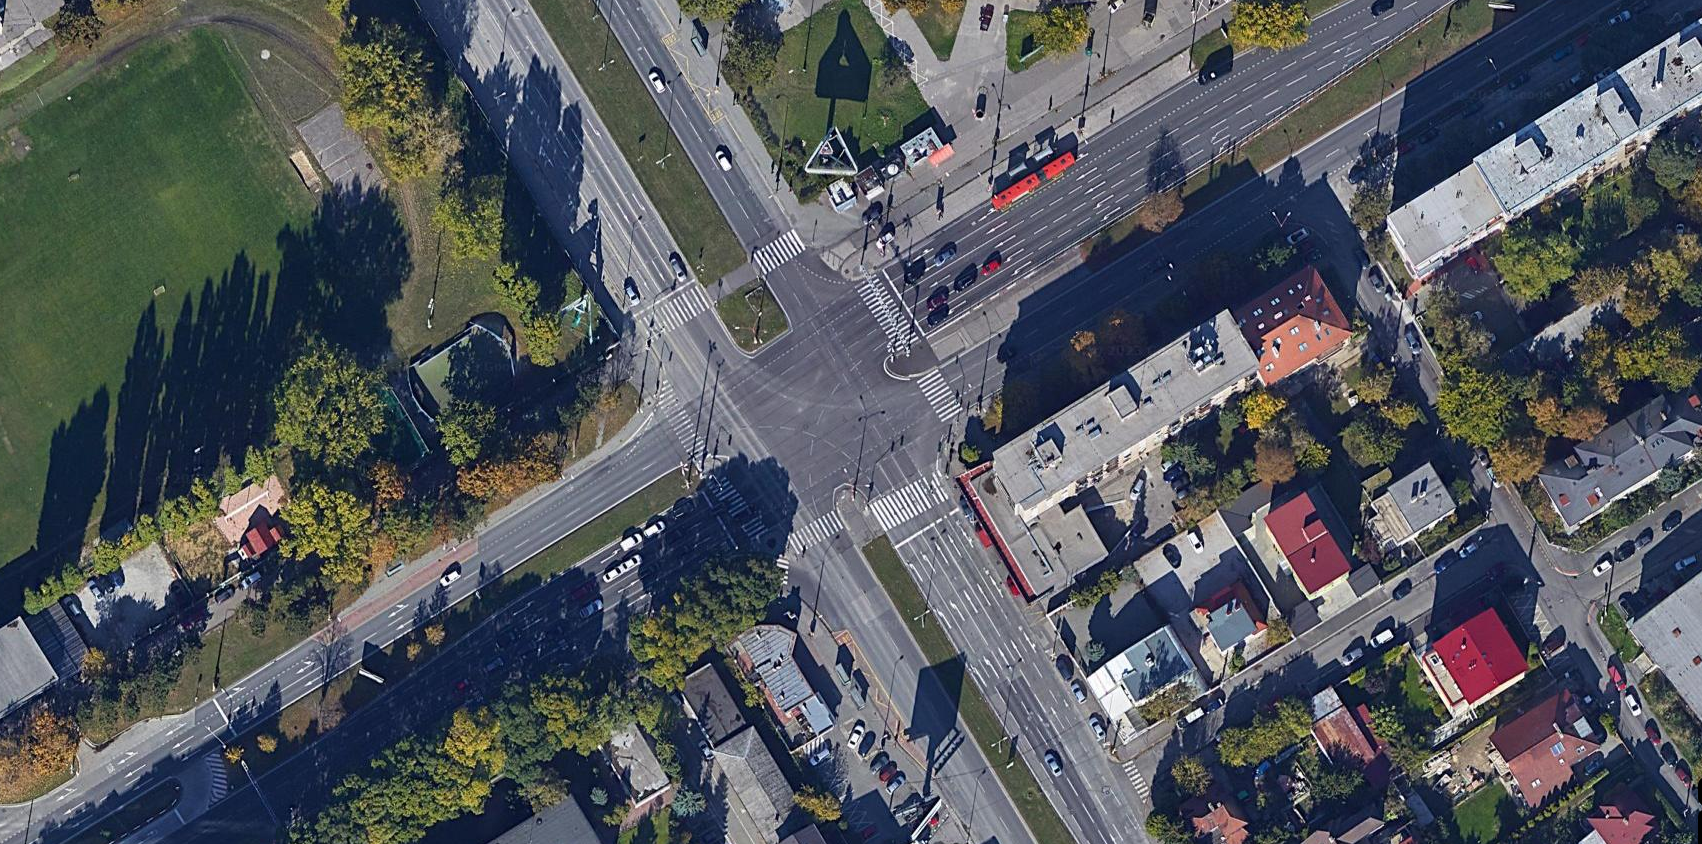
\includegraphics[width=\textwidth]{bajkalska}}
	\only<2>{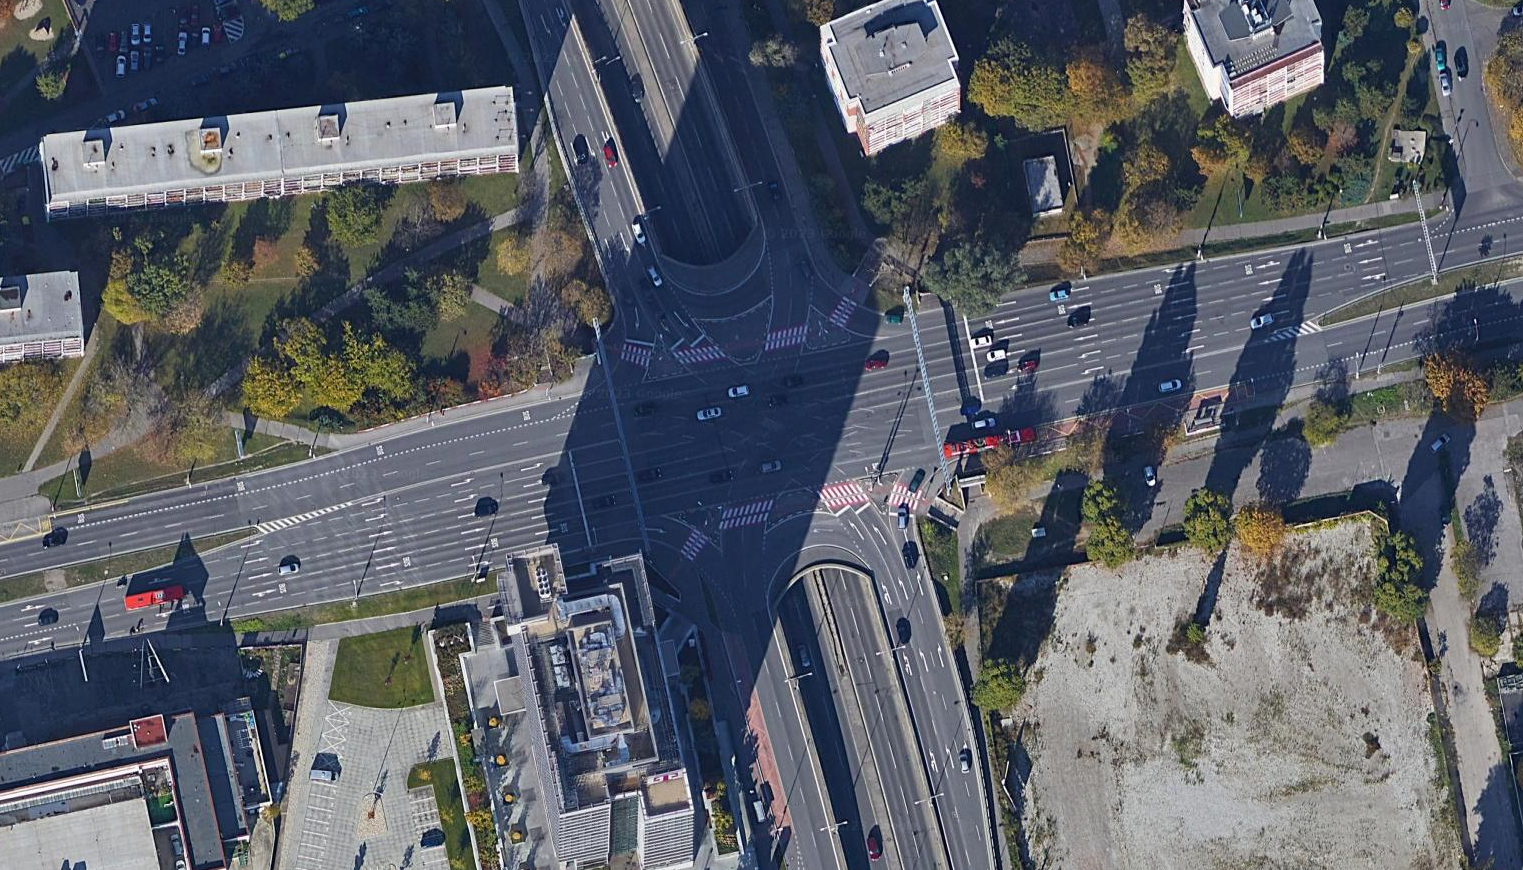
\includegraphics[width=\textwidth]{prievozska}}
\end{frame}

\begin{frame}
	\frametitle{Highways in the city - Wat this America??????}
	\only<1>{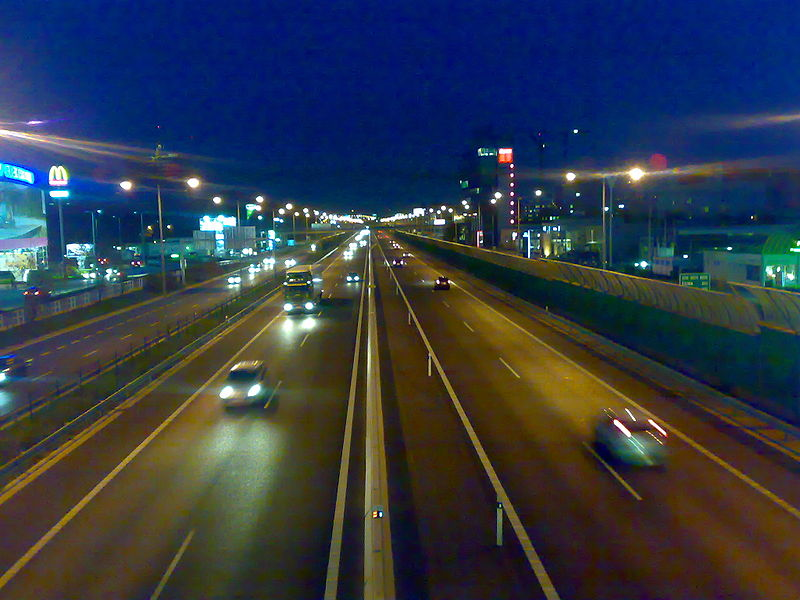
\includegraphics[width=0.8\textwidth]{D1}}
	\only<2>{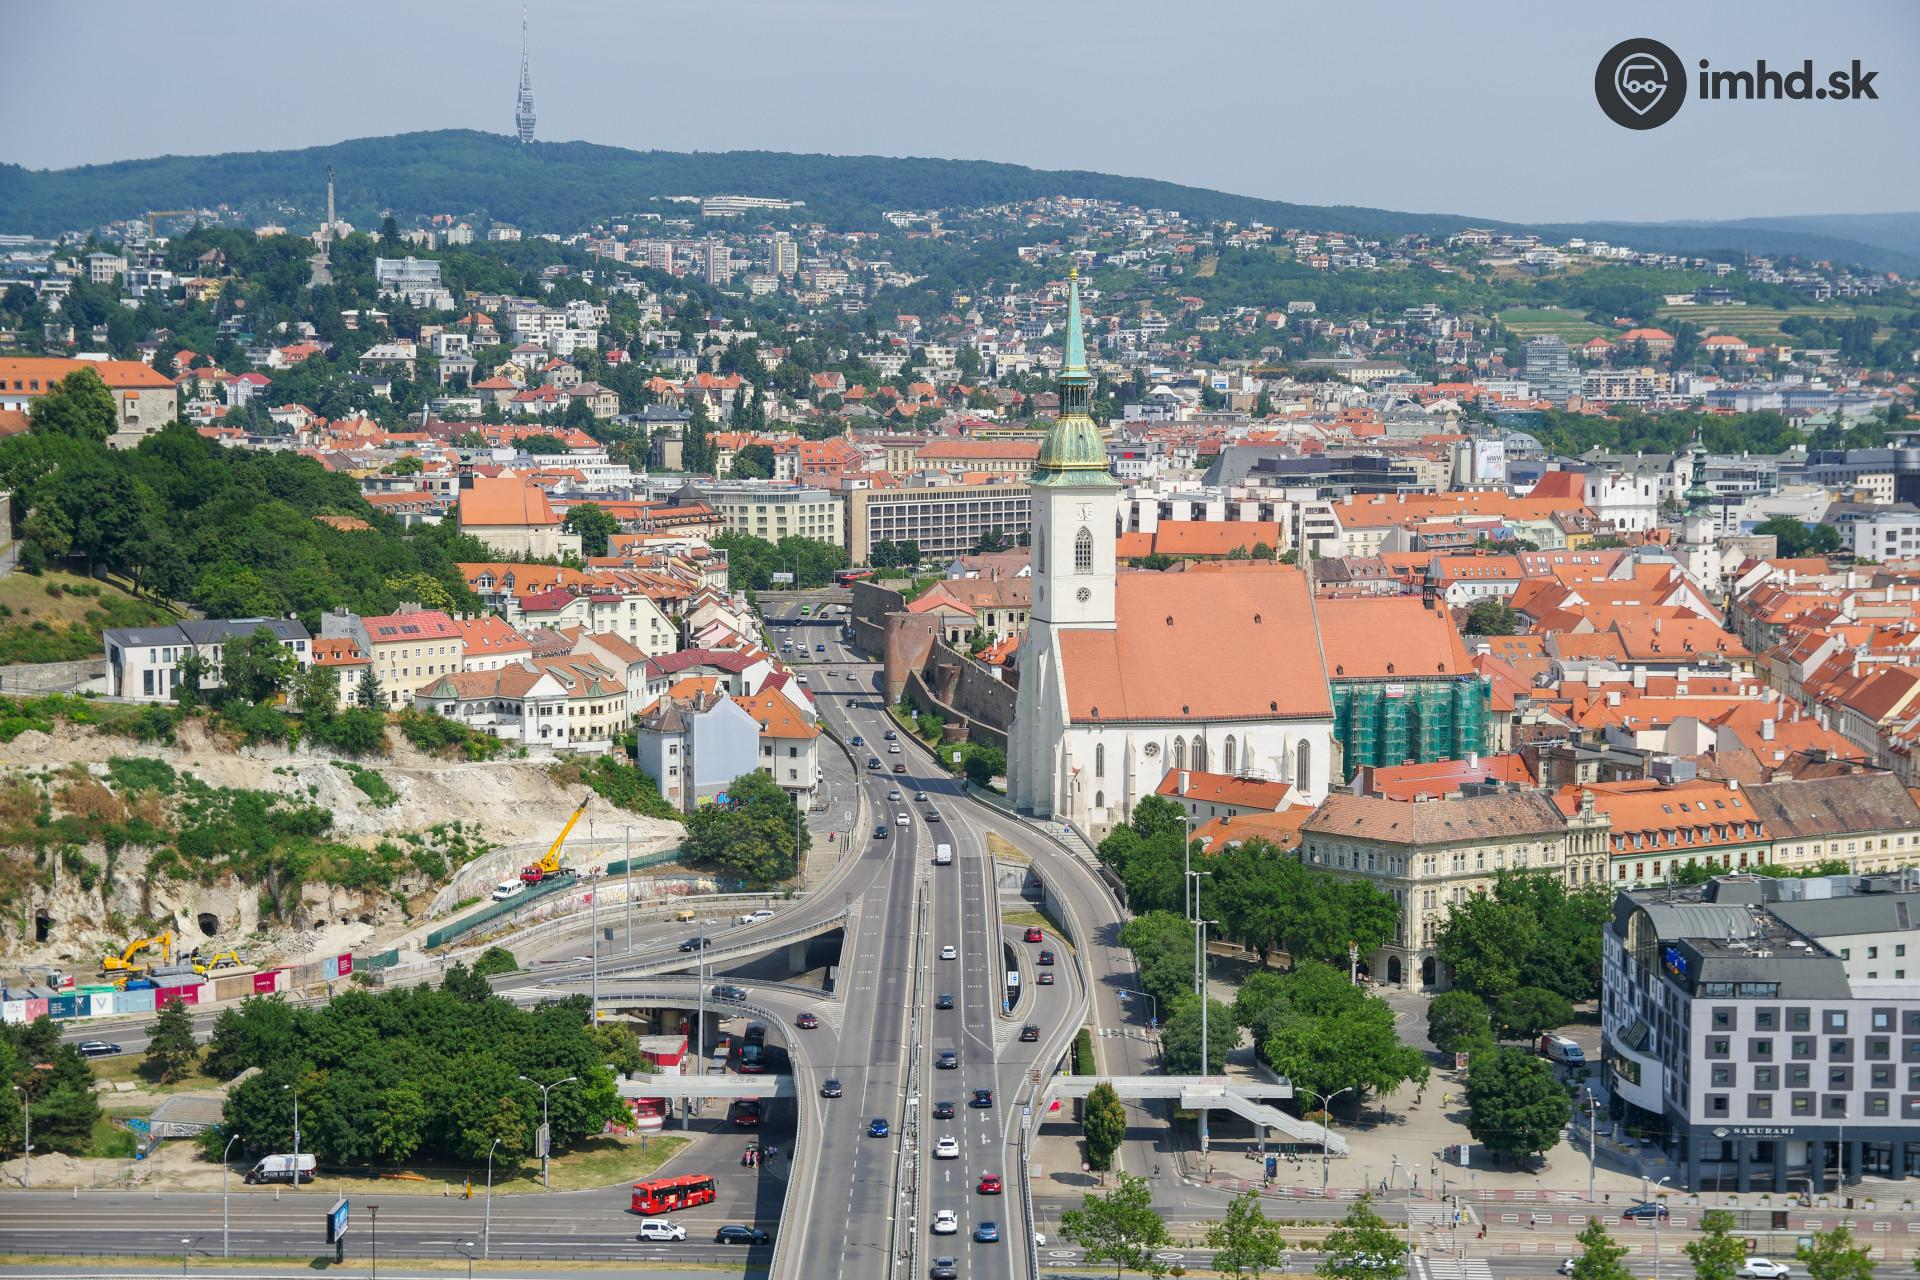
\includegraphics[width=0.8\textwidth]{staromestska}}
	\only<3>{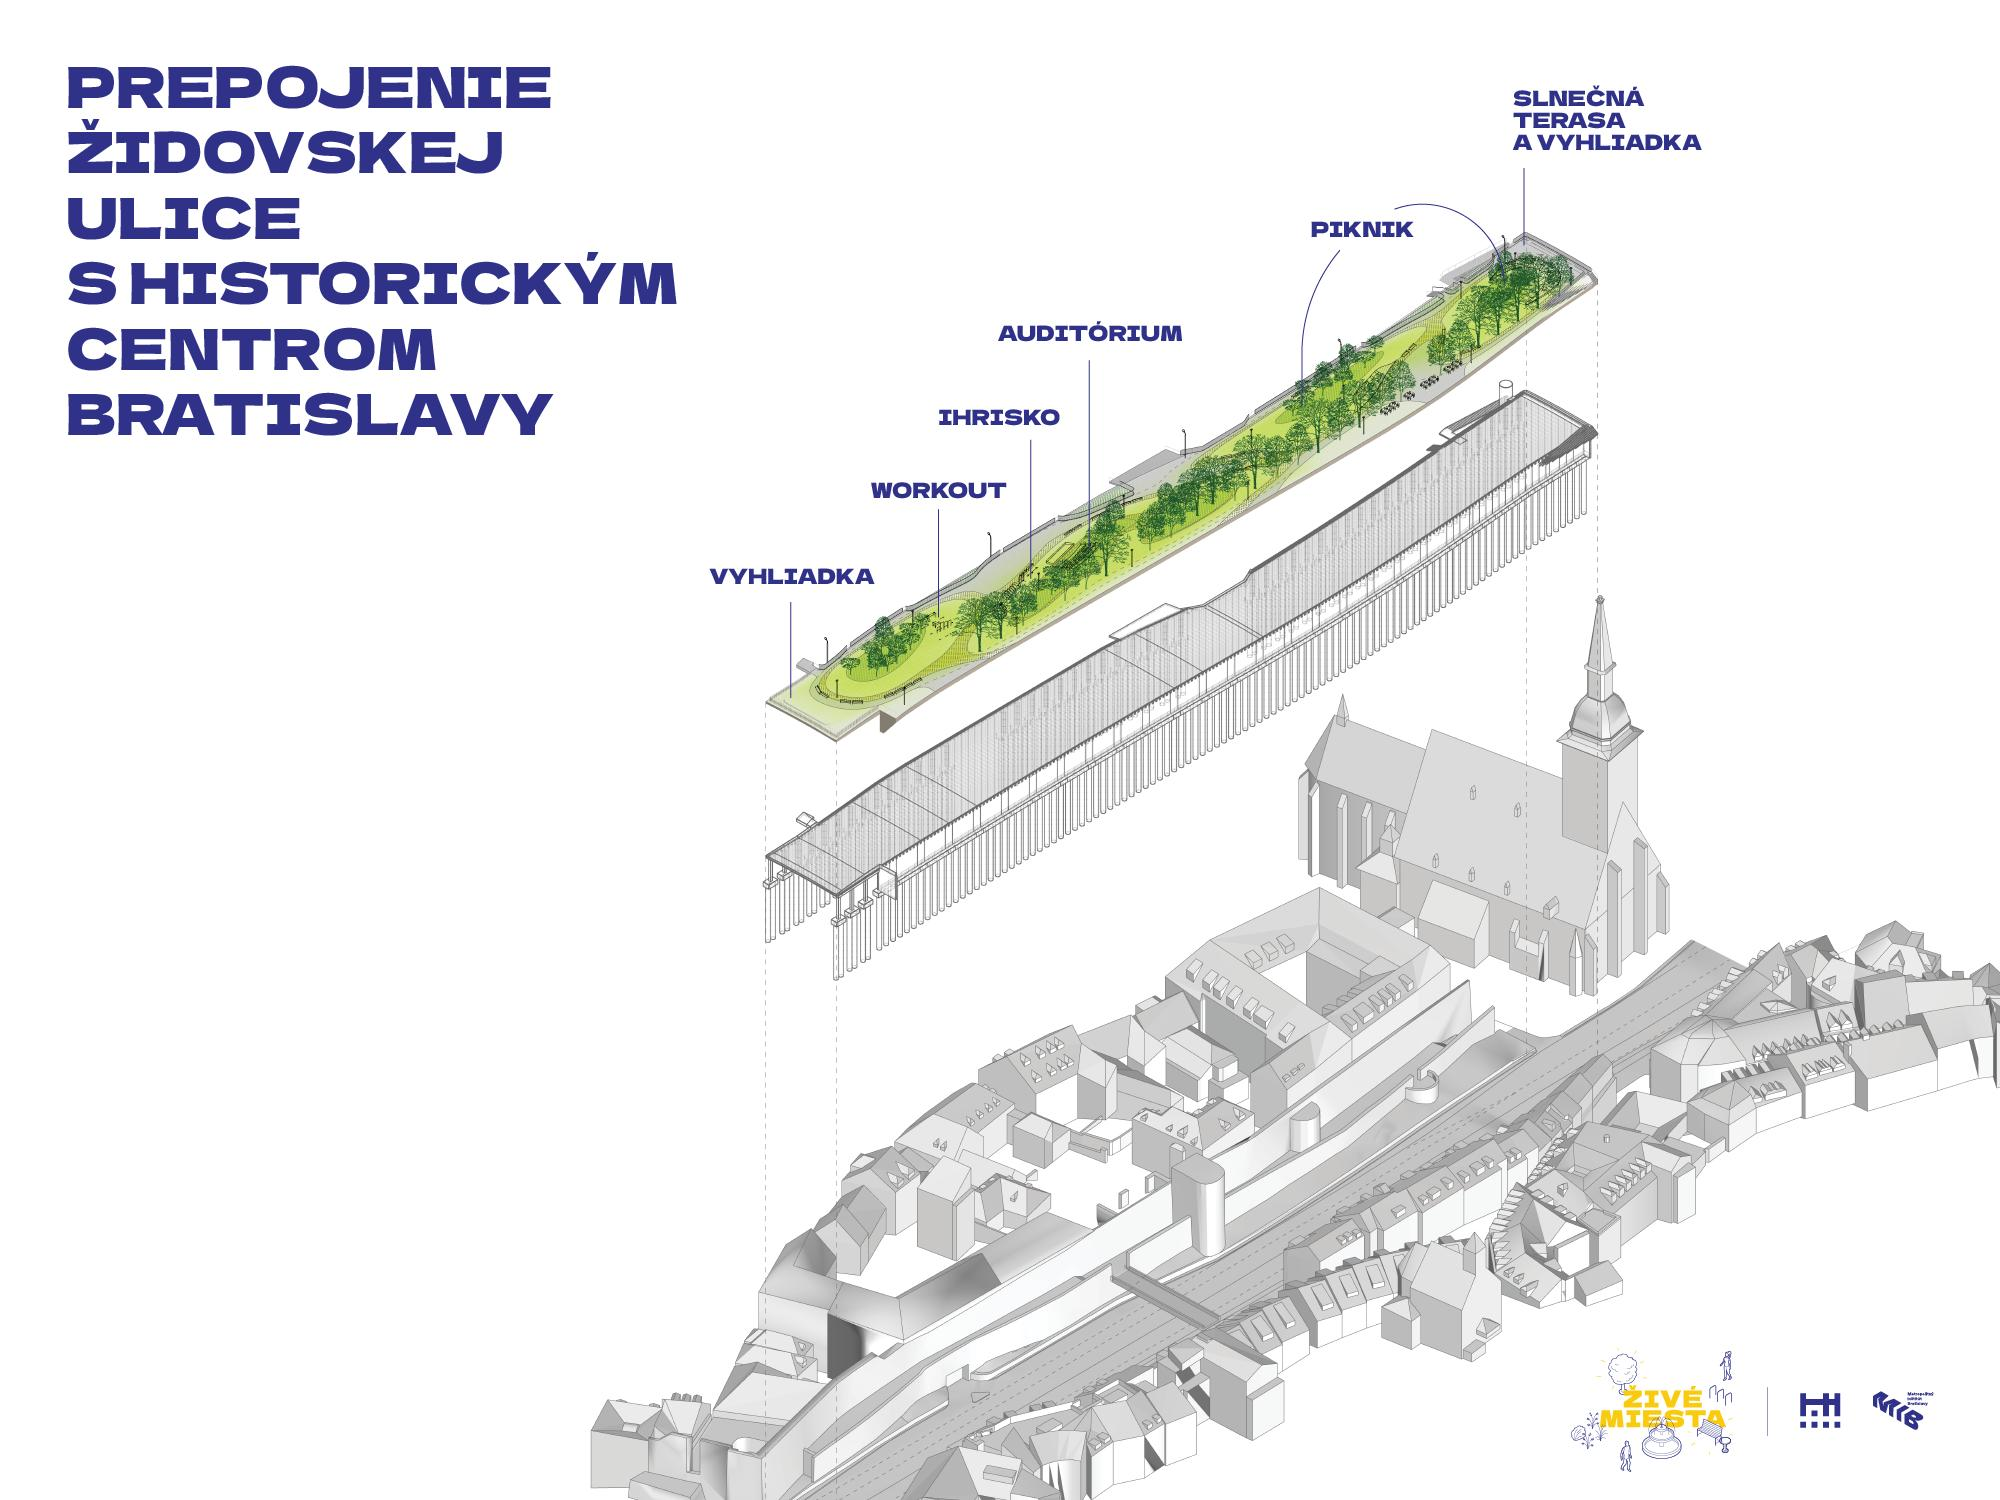
\includegraphics[width=0.8\textwidth]{staromestska-plan}}
\end{frame}

\subsection{Where is Bratislava growing?}

\begin{frame}
	\frametitle{The new downtown}
	\begin{columns}
		\begin{column}{.48\textwidth}
			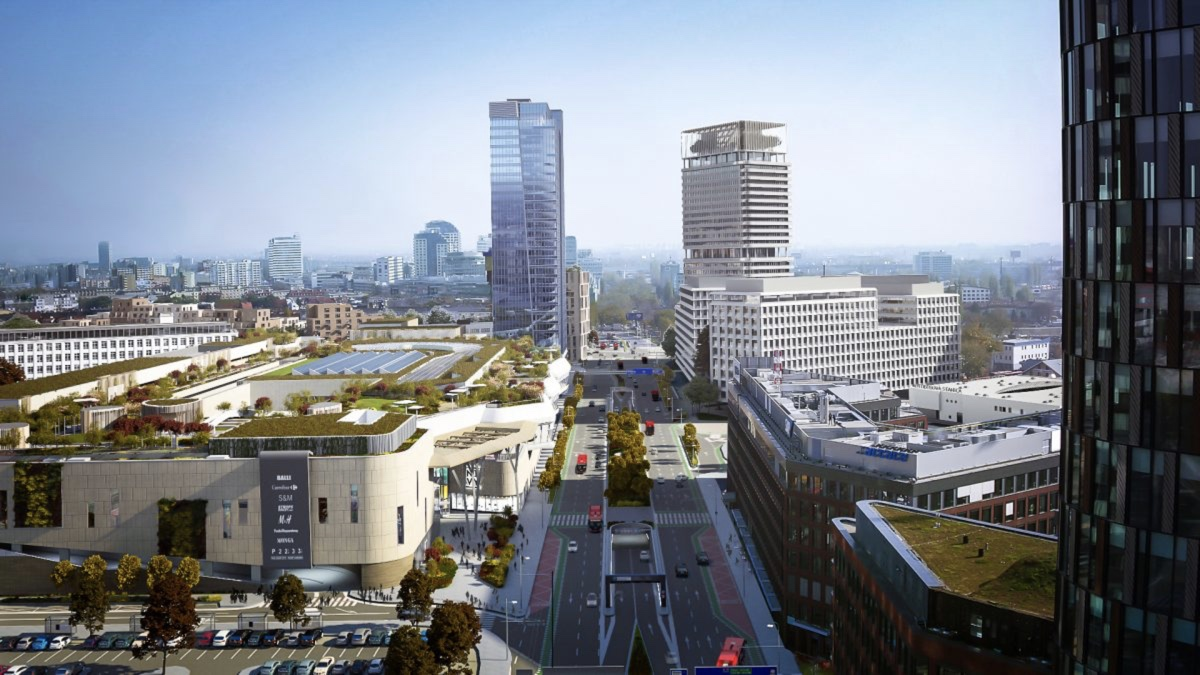
\includegraphics[width=\textwidth]{nivy}\\
			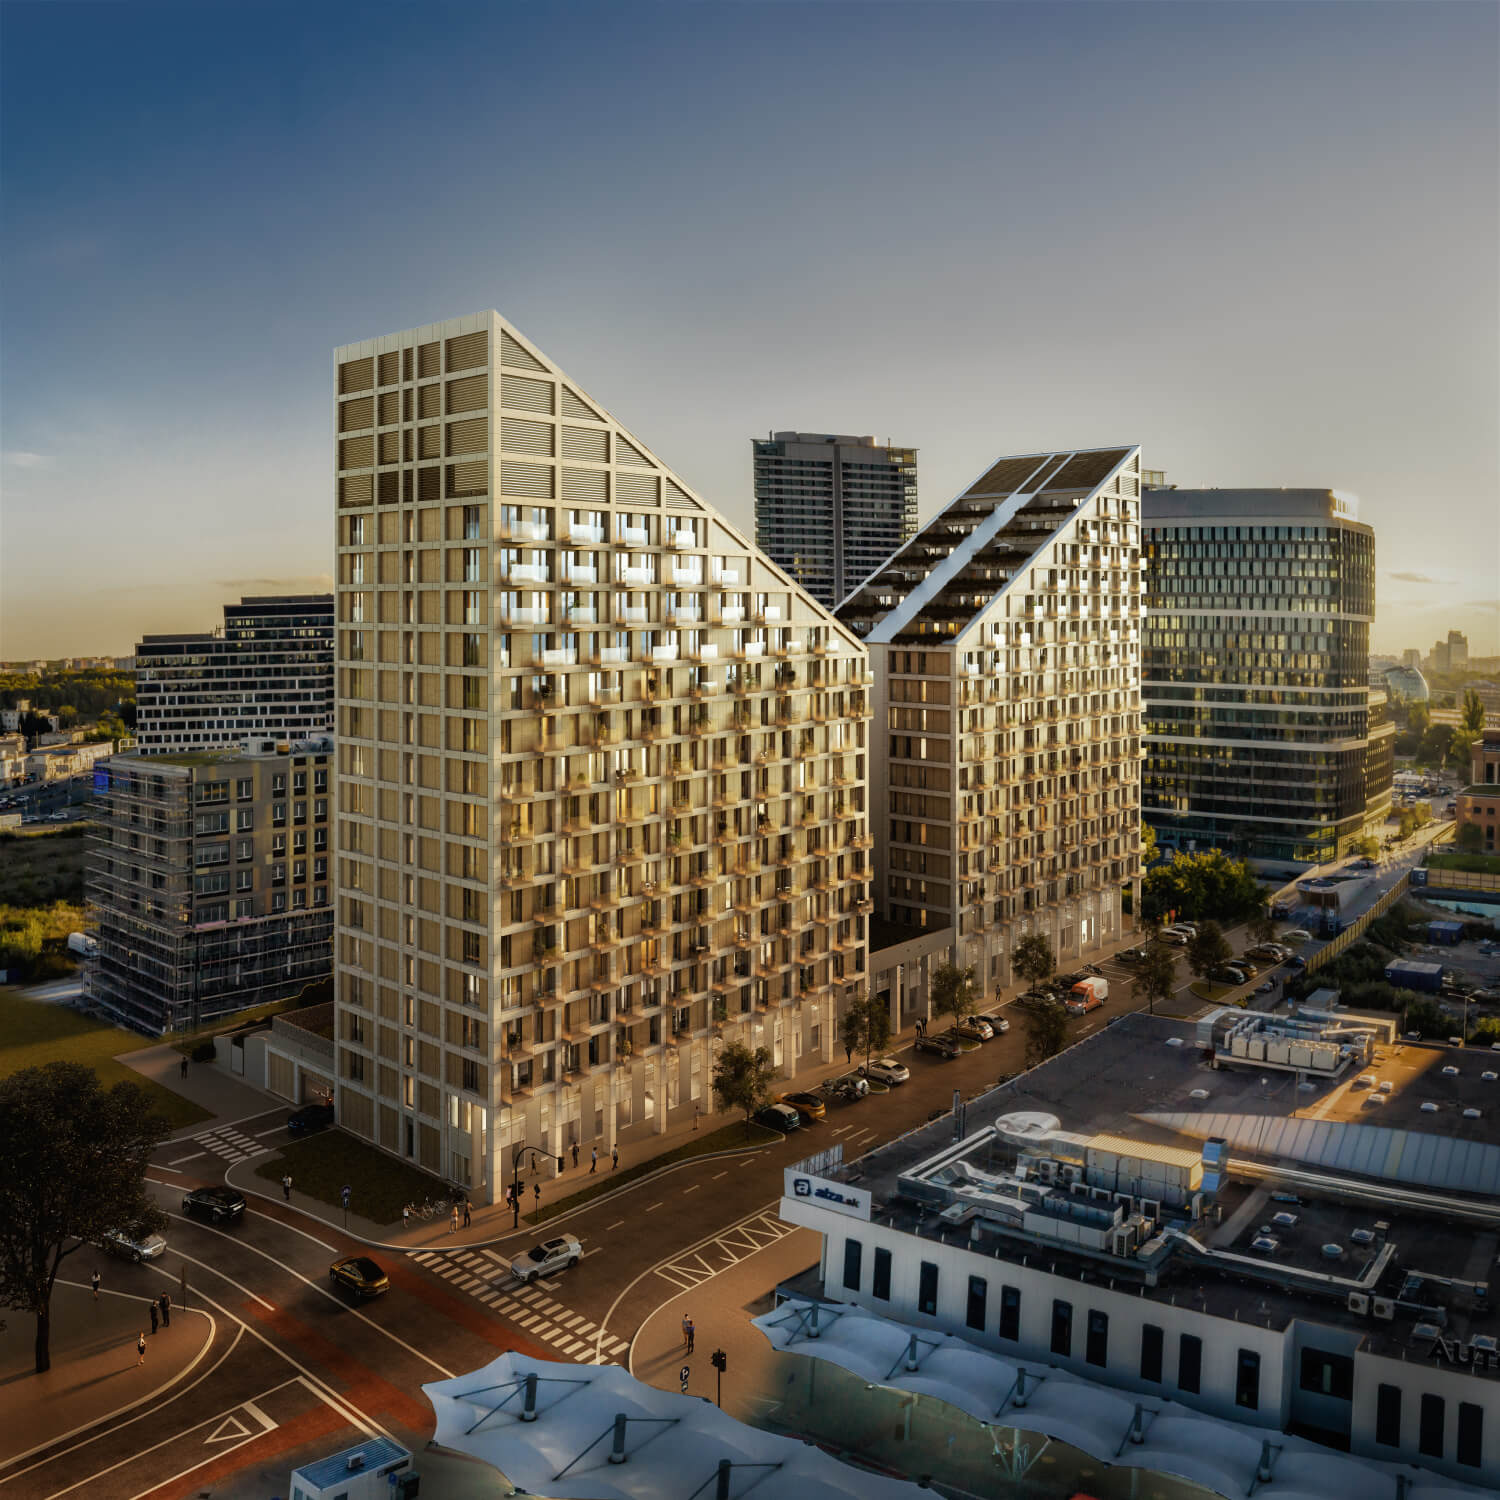
\includegraphics[width=\textwidth]{bottova}
		\end{column}
		\begin{column}{.48\textwidth}
			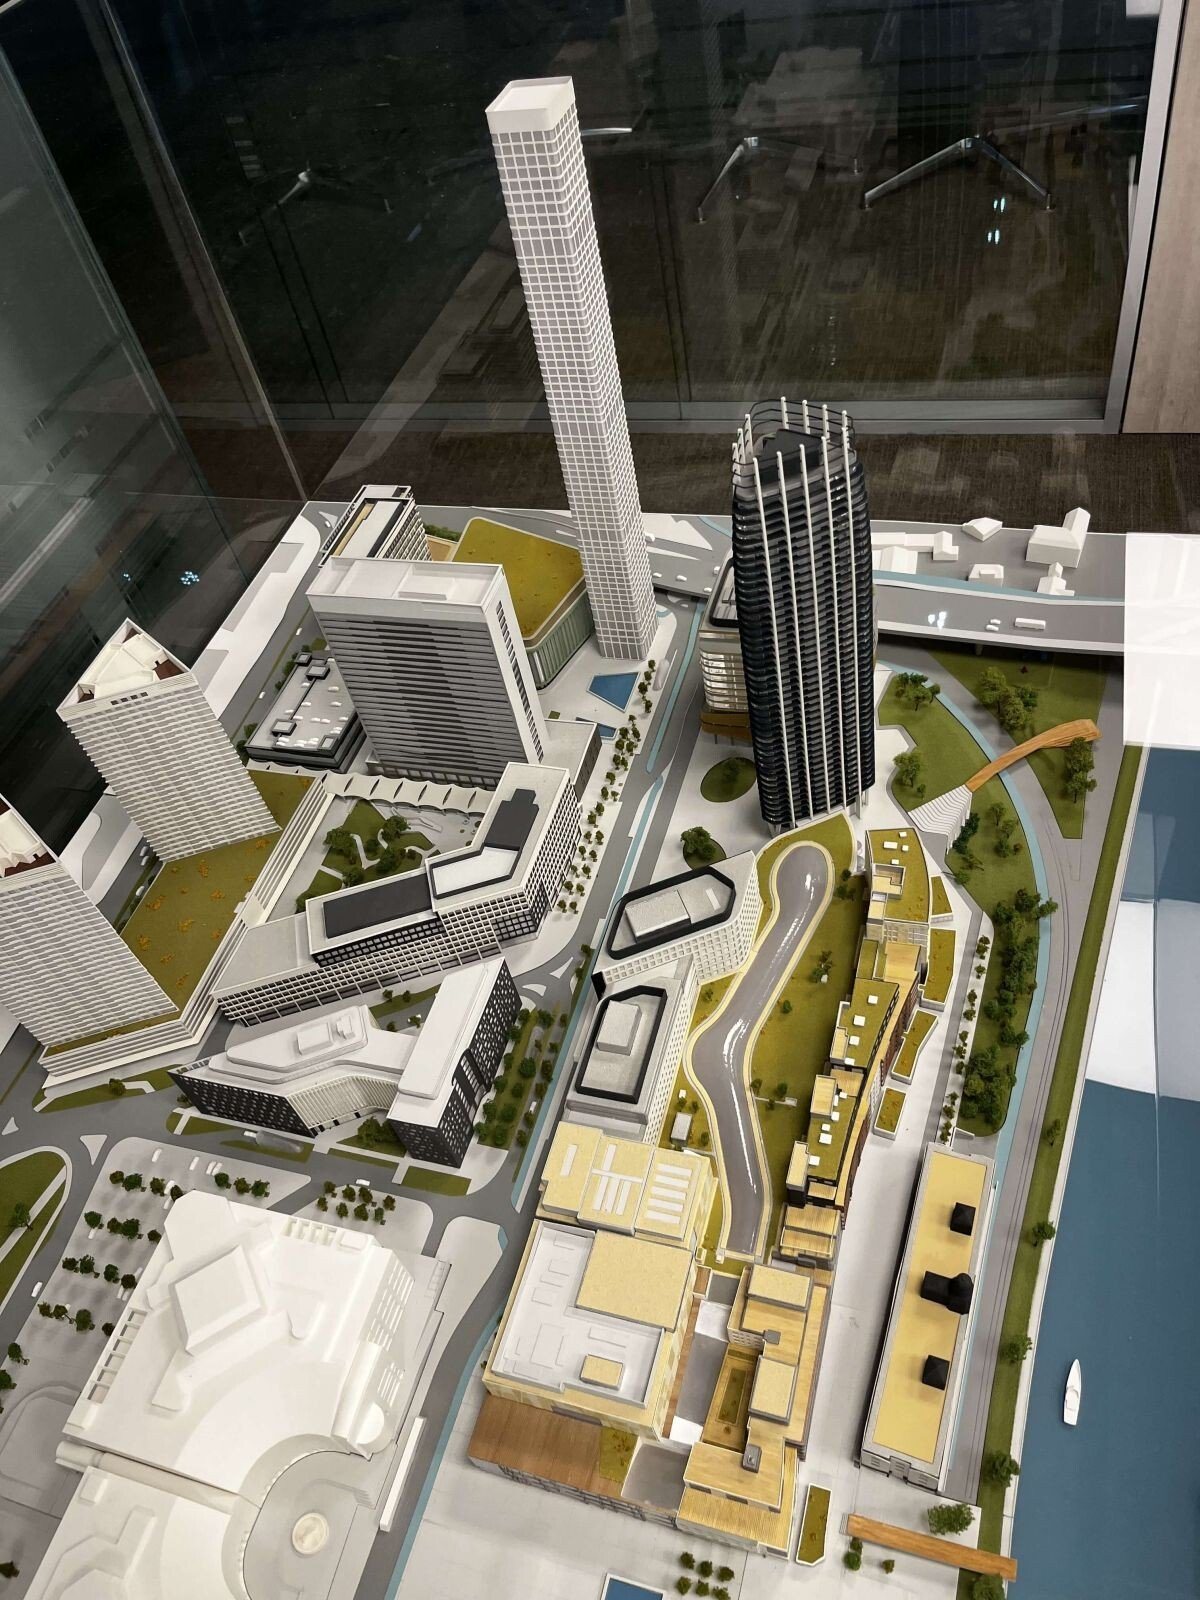
\includegraphics[width=\textwidth]{downtown-1}
		\end{column}
	\end{columns}
\end{frame}

\begin{frame}
	\frametitle{The new downtown}
	\framesubtitle{The infamous tram}

	\begin{columns}
		\begin{column}{.48\textwidth}
			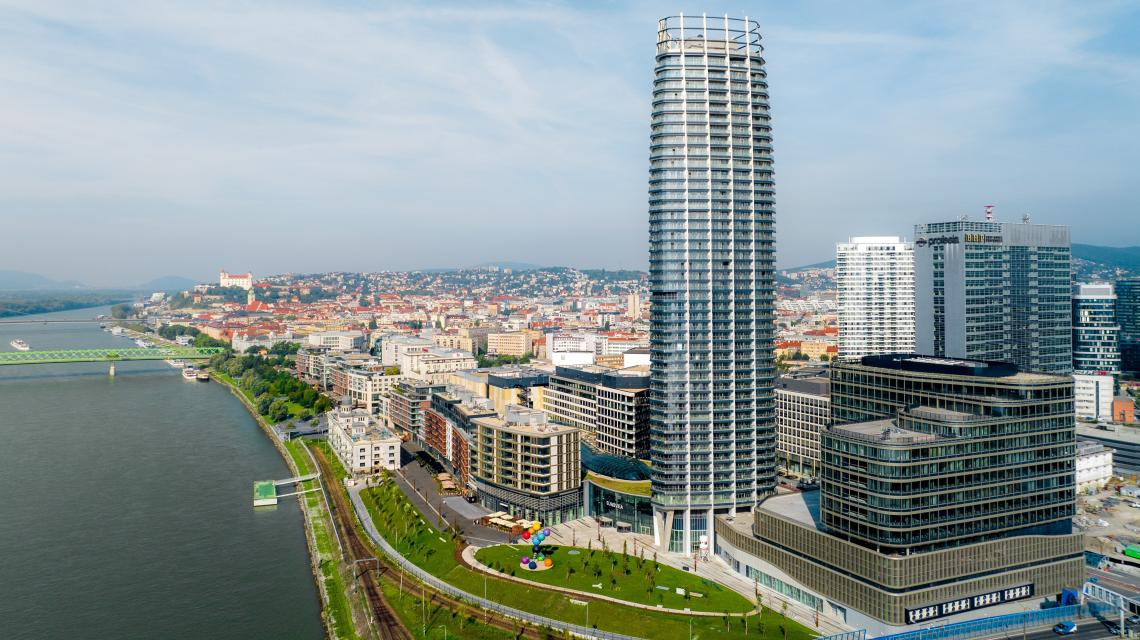
\includegraphics[width=\textwidth]{eurovea-tower}
		\end{column}
		\begin{column}{.48\textwidth}
			\only<1>{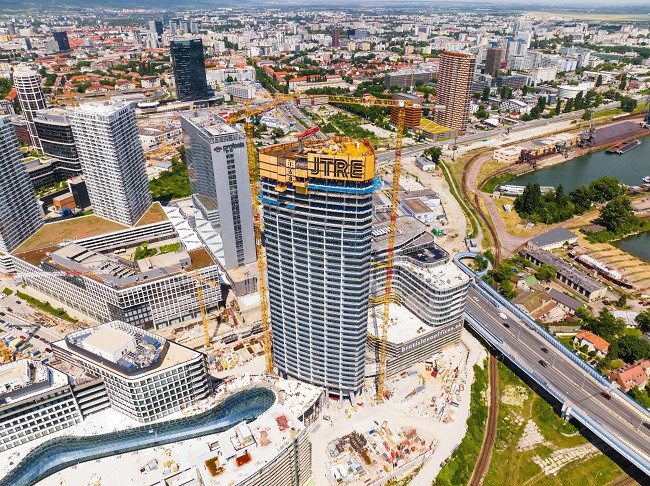
\includegraphics[width=\textwidth]{jtre}}
			\only<2>{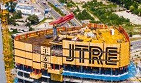
\includegraphics[width=\textwidth]{jtre-zoomed}}
		\end{column}
	\end{columns}

	\vspace{1em}

	\only<3>{\url{https://www.youtube.com/watch?v=8ZU-MiCpAv0\&ab\_channel=JTRE}}
\end{frame}

\begin{frame}
	\frametitle{How transit generates wealth}

	\begin{columns}
		\begin{column}{.45\textwidth}
			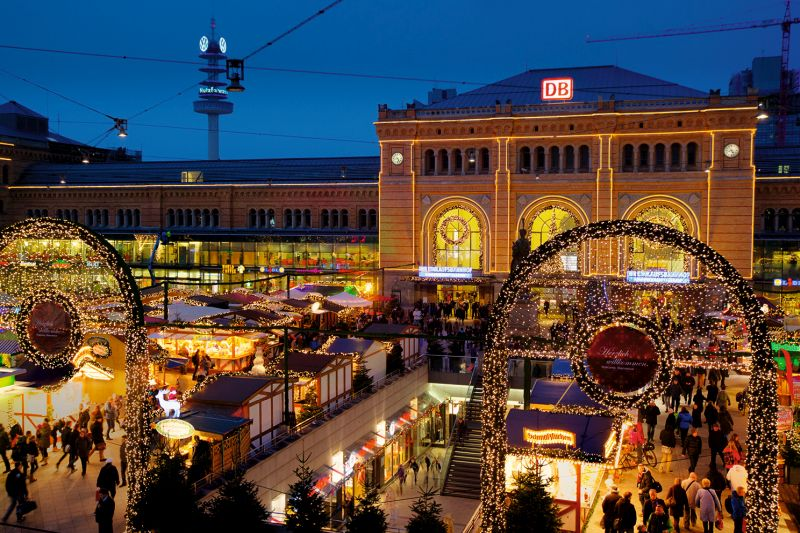
\includegraphics[width=\textwidth]{hannover}\\
			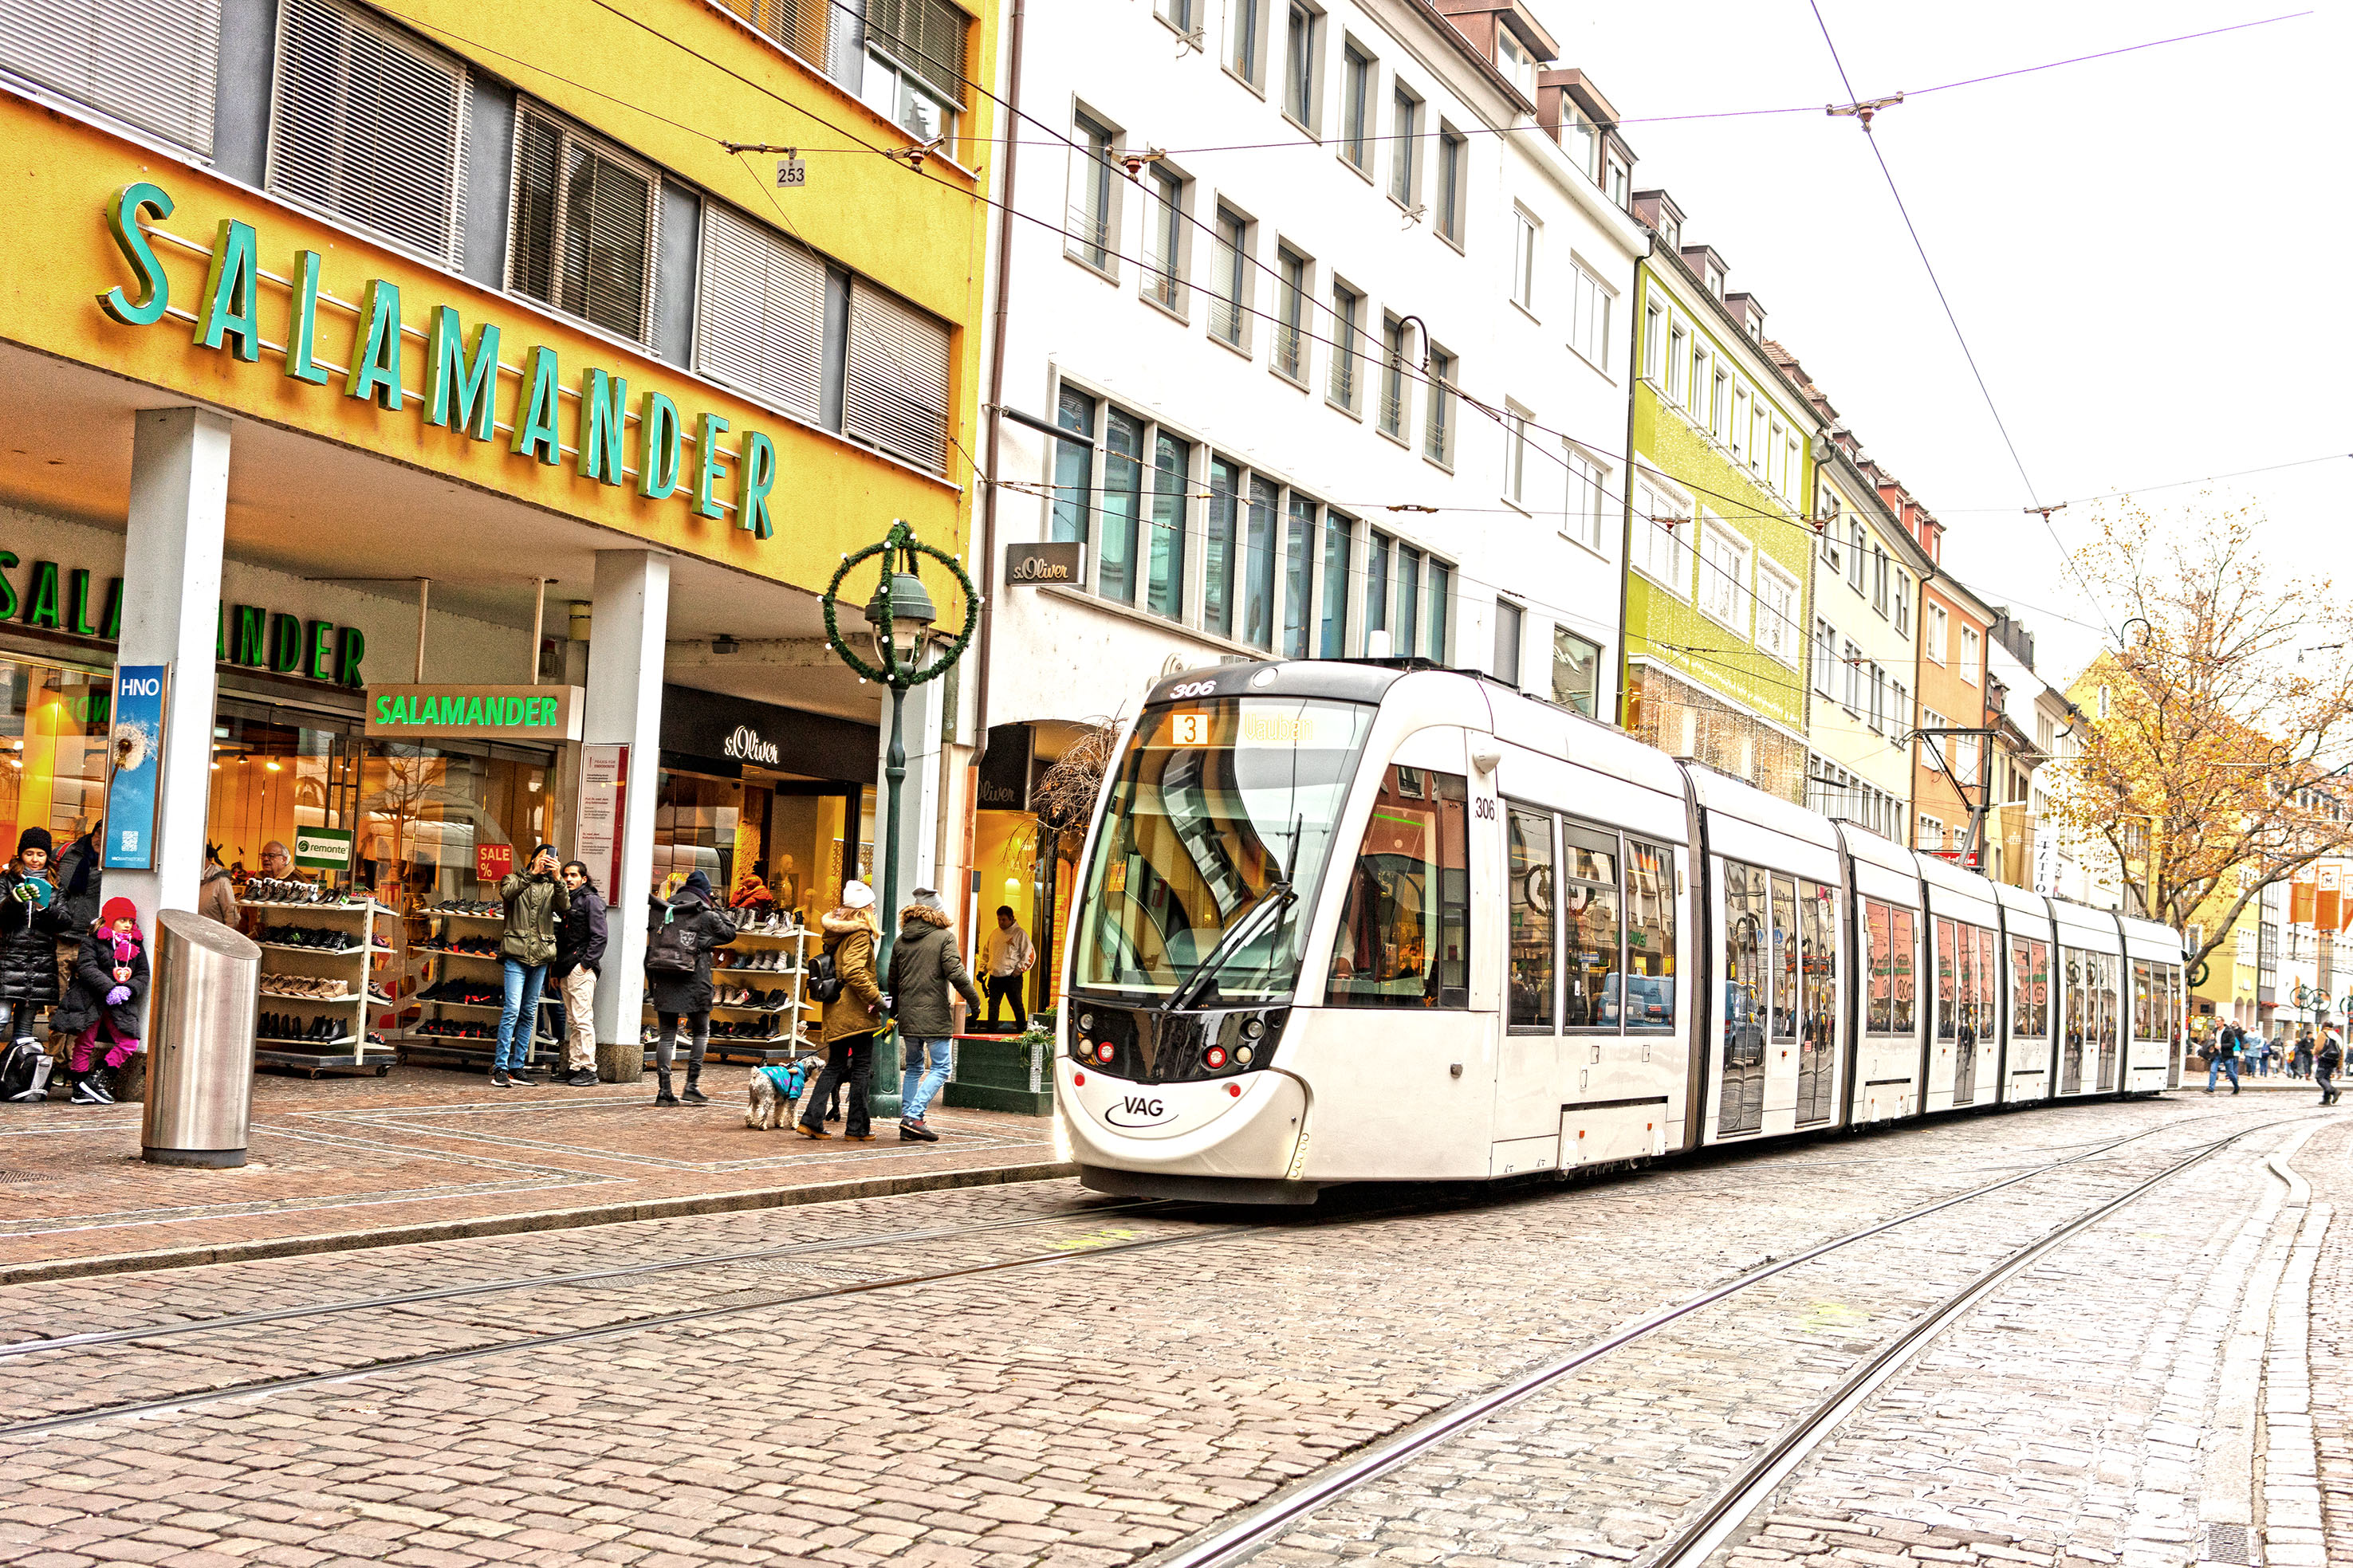
\includegraphics[width=\textwidth]{freiburg}
		\end{column}
		\begin{column}{.45\textwidth}
			{\Large What to strive for}\\[.5em]
			\begin{enumerate}
				\item \underline{Don't build big at once}
				\item Build on \underline{demand}
				\item Connect only places that need connecting (duh)
			\end{enumerate}
		\end{column}
	\end{columns}
\end{frame}

\subsection{Trams}

\begin{frame}
	\frametitle{Transportation - Trams}
	\framesubtitle{Basic facts}

	\begin{enumerate}
		\item 42km of rail (Brno has 70km)
		\item 211 vehicles (Brno has 305)
		\item 5 lines (Brno has 11)
		\item frequent times
		\item good vehicles
	\end{enumerate}
\end{frame}

\begin{frame}
	\frametitle{Transportation - Trams}
	\framesubtitle{Petržalka will have a tram}
	\centering
	
	\only<1>{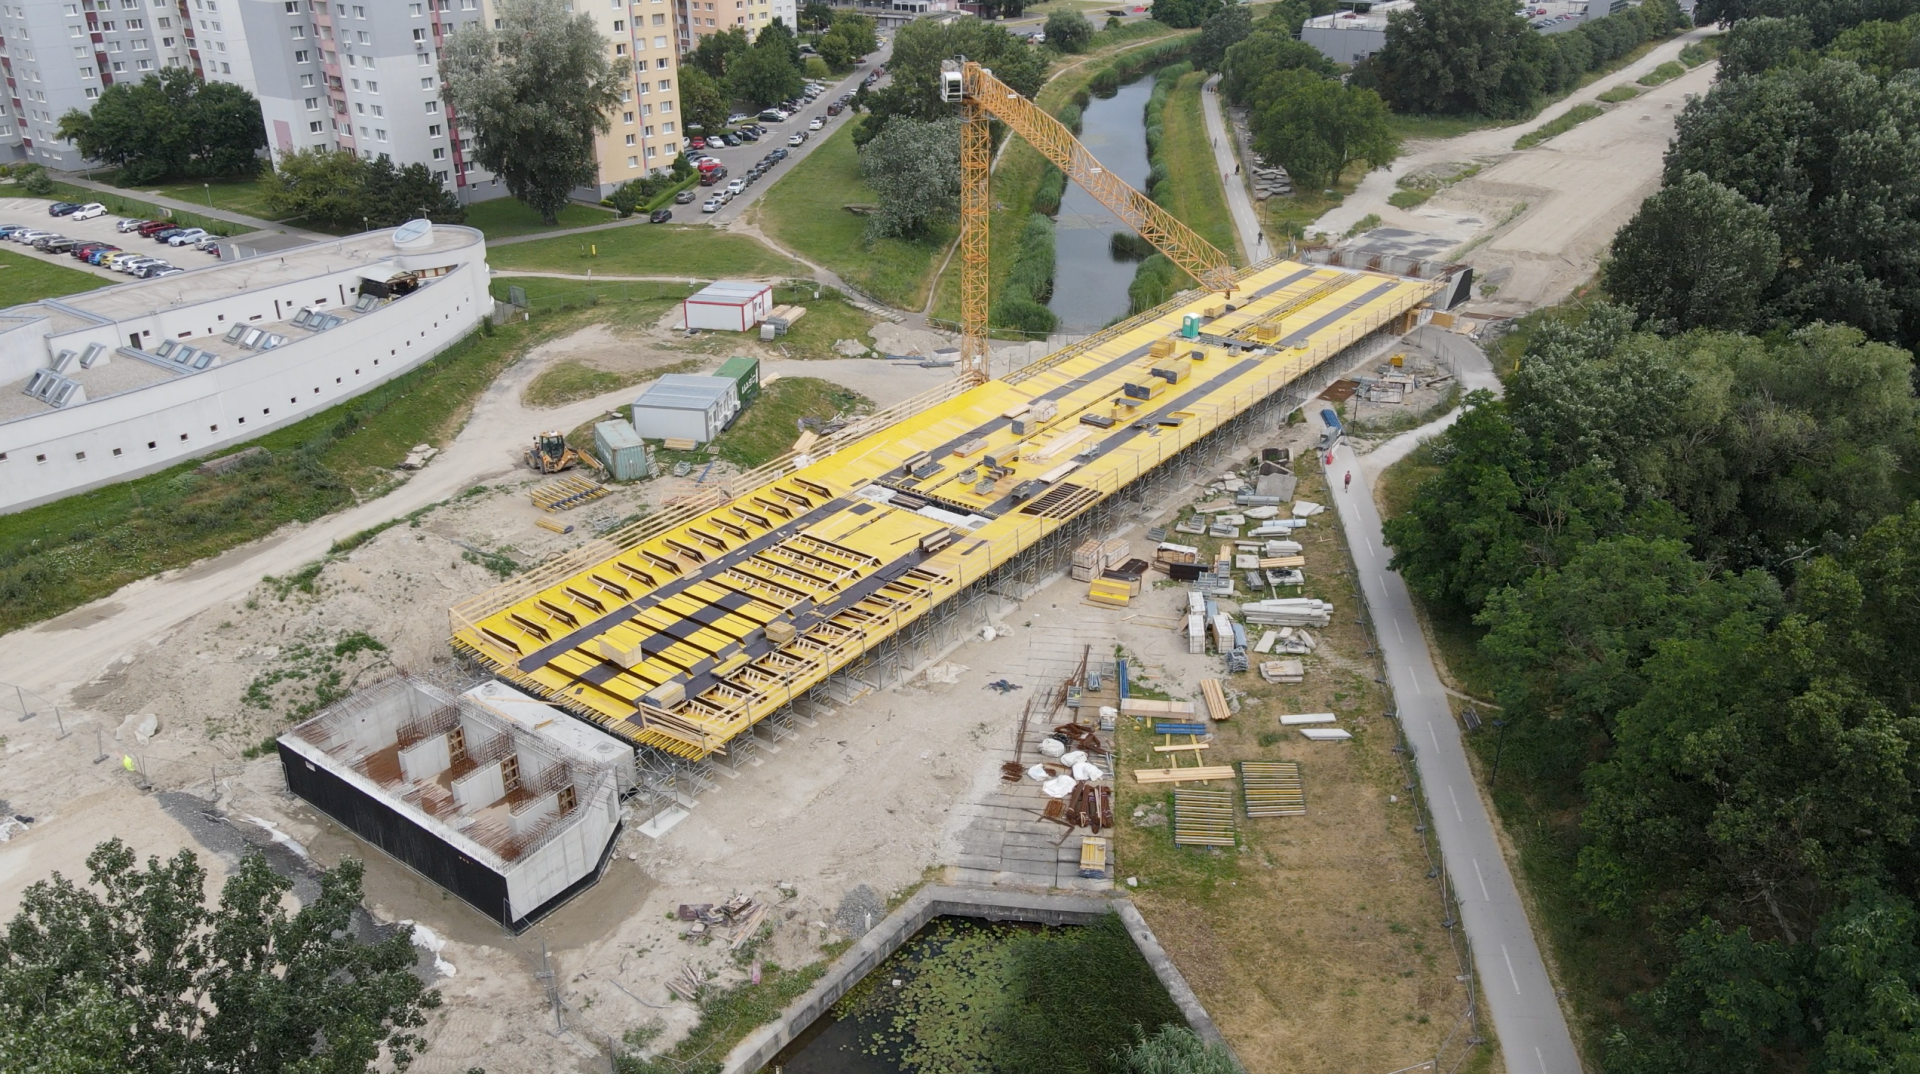
\includegraphics[width=.9\textwidth]{petrzalska-elektricka-1}}
	\only<2>{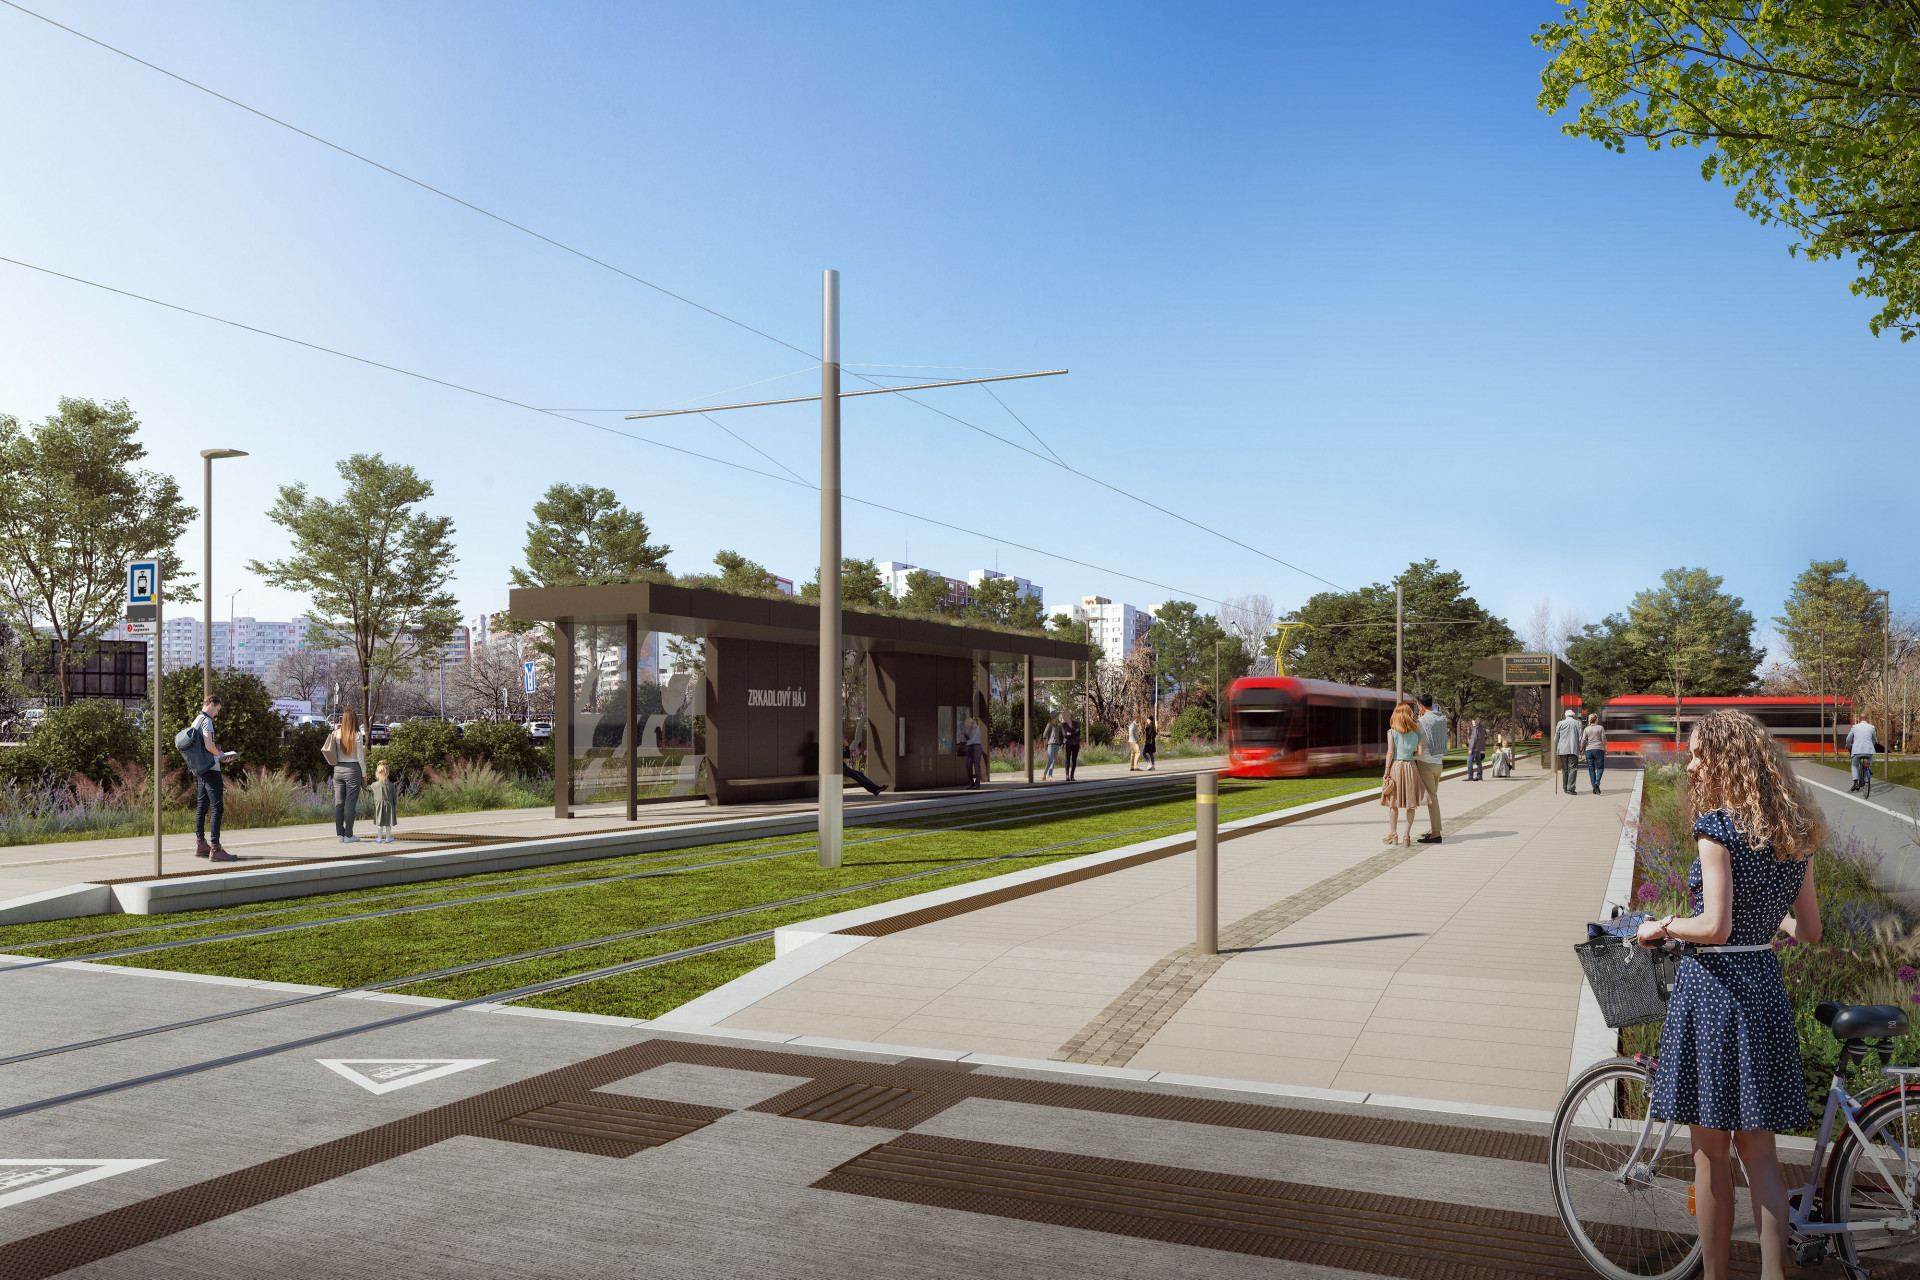
\includegraphics[width=.9\textwidth]{petrzalska-elektricka-2}}
	\pause
	\only<3>{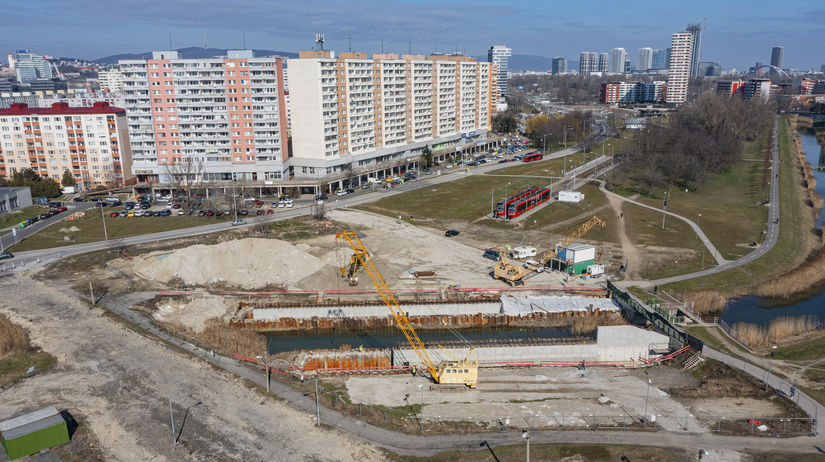
\includegraphics[width=.9\textwidth]{petrzalska-elektricka-3}}
	\pause
	\only<4>{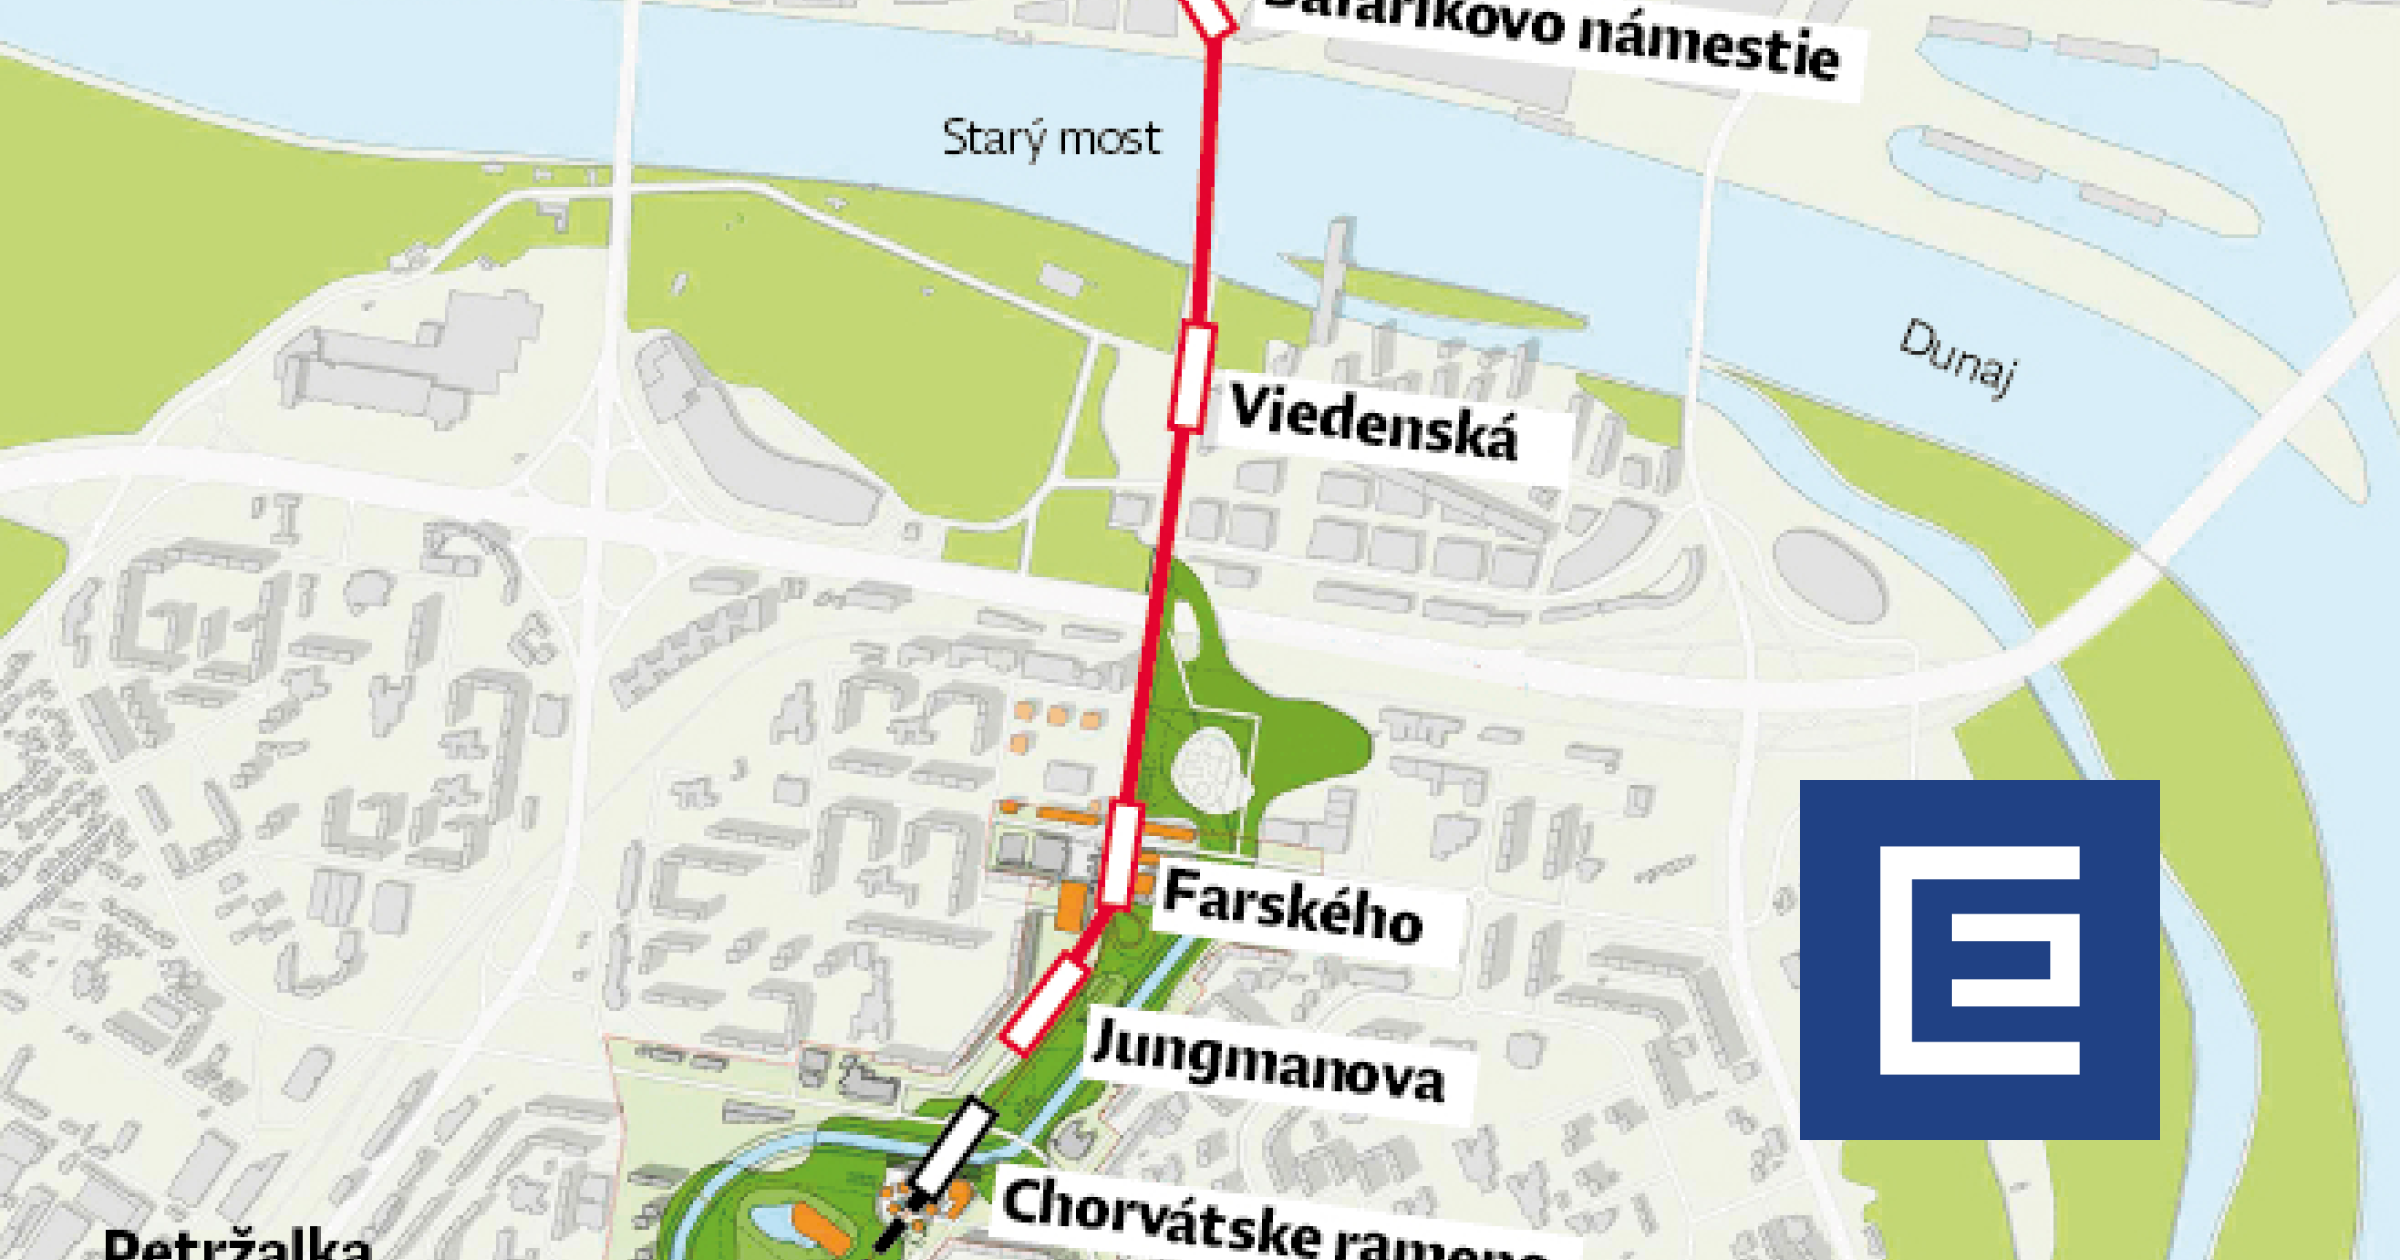
\includegraphics[width=.9\textwidth]{petrzalska-elektricka-4}}
	\pause
	\only<5>{
\includegraphics[width=.9\textwidth]{petrzalska-elektricka-vallo}}
\end{frame}

\subsection{Trains...}
\subsection{How are trains done elsewhere}

\begin{frame}
	\frametitle{What we need: S-Bahn}

	\centering
	\begin{columns}
		\begin{column}{.5\textwidth}
			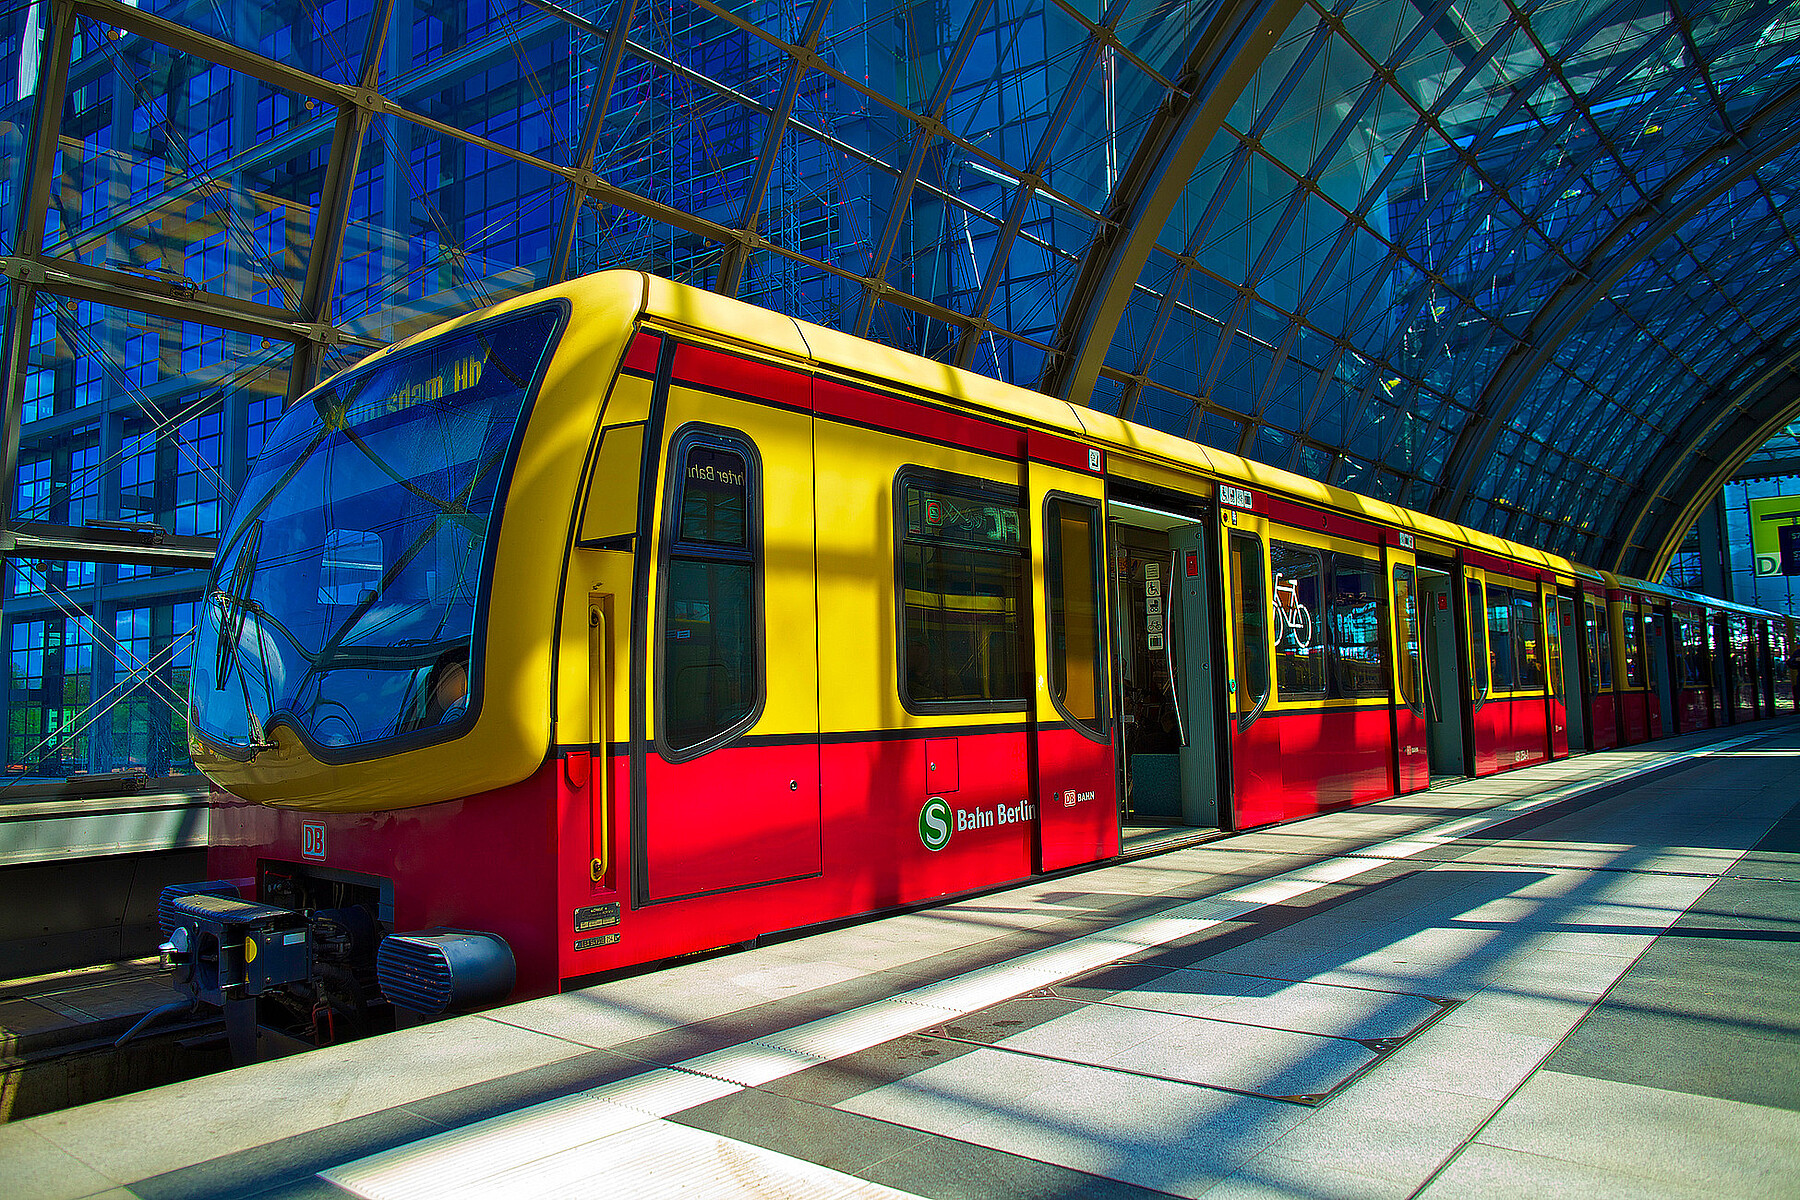
\includegraphics[width=\textwidth]{sbahn-1}
		\end{column}
		\begin{column}{.5\textwidth}
			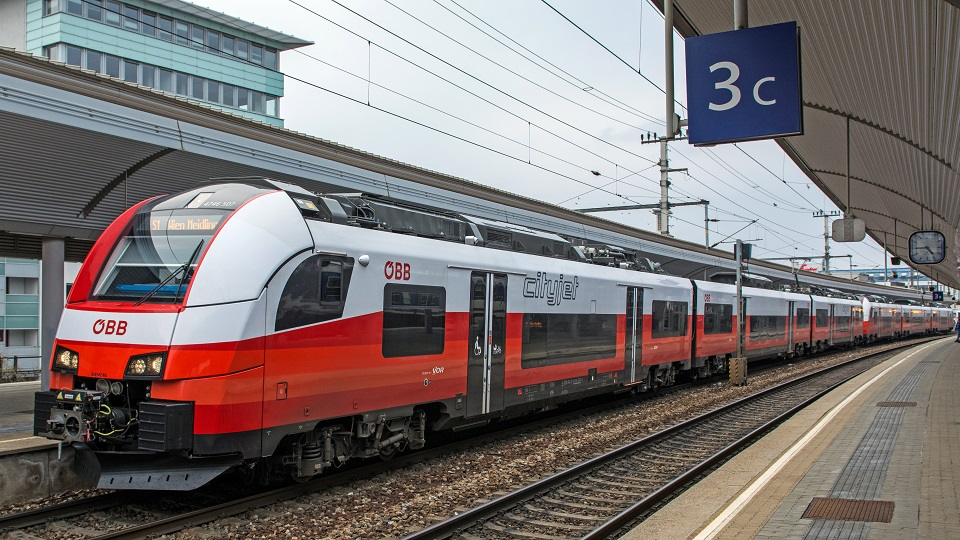
\includegraphics[width=\textwidth]{sbahn-2}
		\end{column}
	\end{columns}
	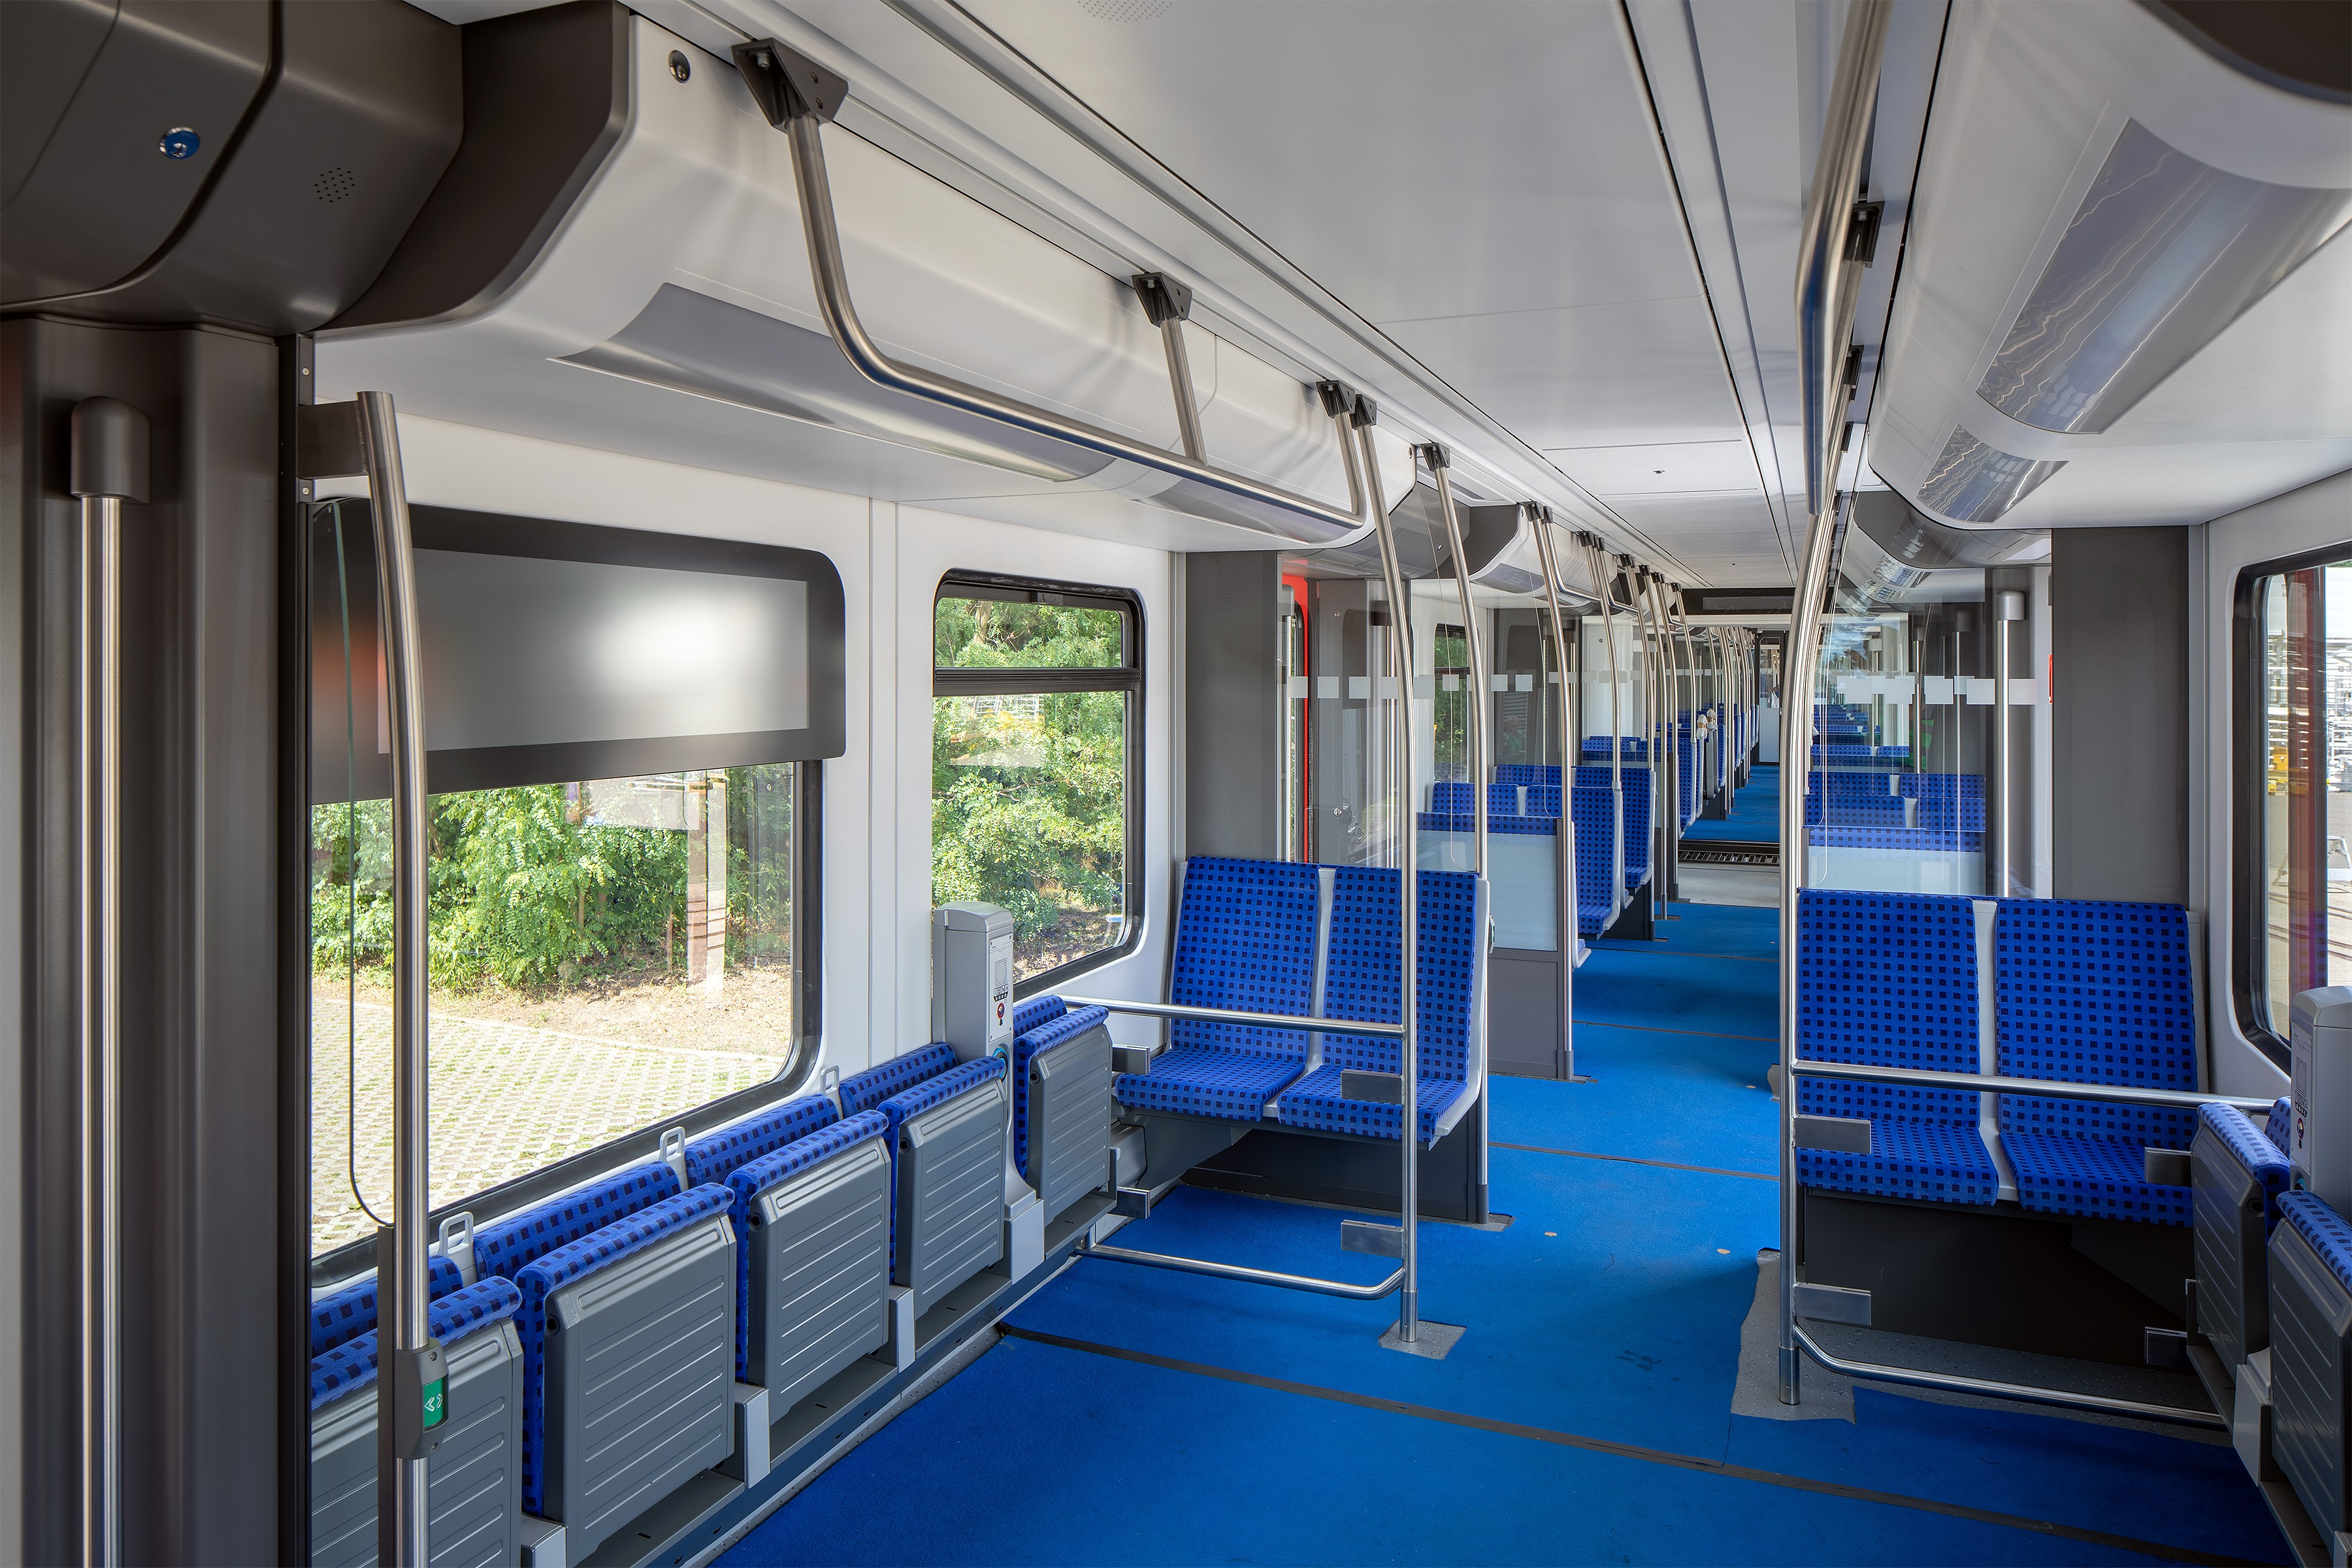
\includegraphics[height=0.4\textheight]{sbahn-3}
\end{frame}

\begin{frame}
	\frametitle{S-Bahn in Deutschland}
	
	\centering
	\only<1>{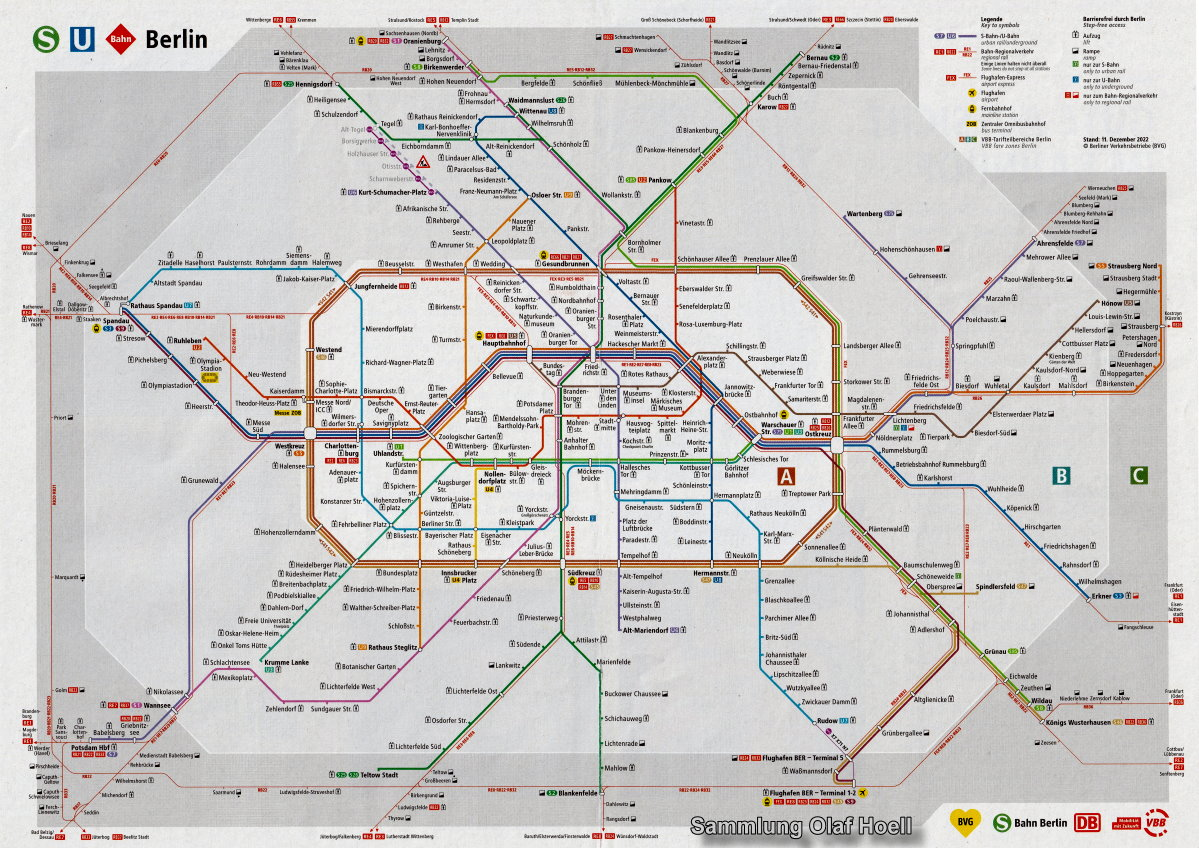
\includegraphics[width=\textwidth]{sbahn-netz-berlin}}
	\only<2>{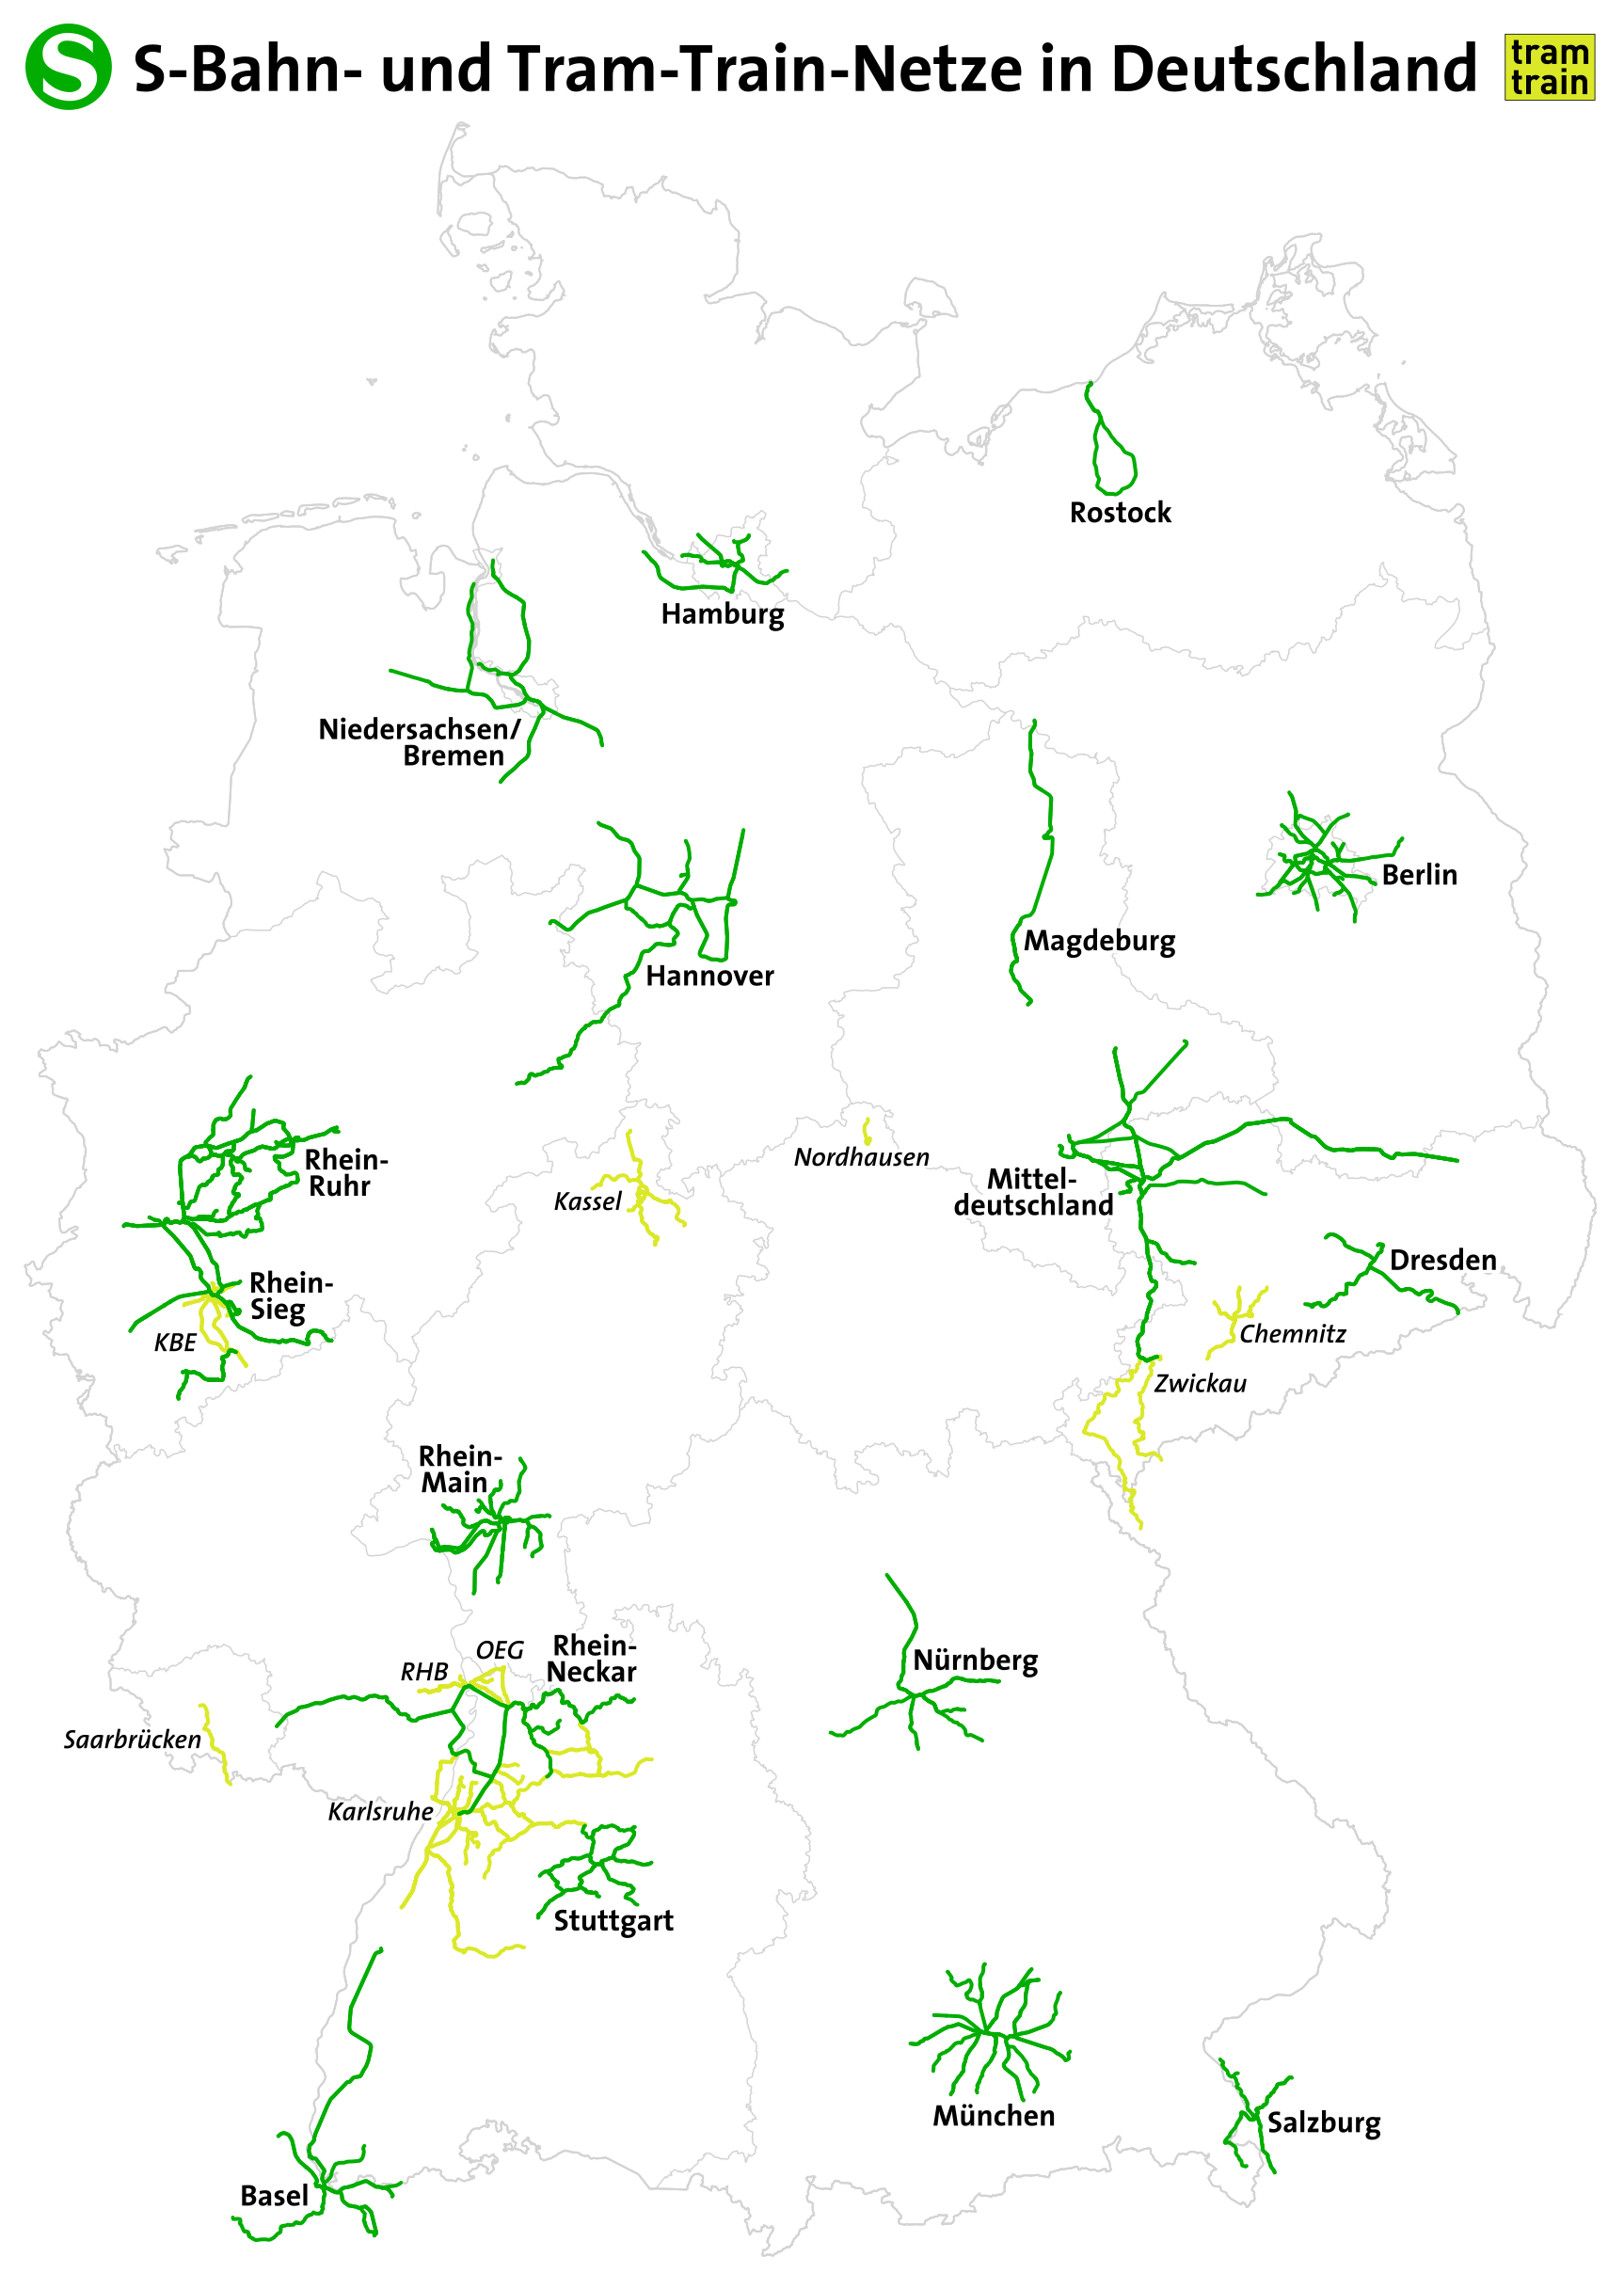
\includegraphics[height=.7\textheight]{sbahn-netz-deutschland}}
\end{frame}

\begin{frame}
	\frametitle{Example of how to generate wealth with transit - Hannover Hauptbahnof}
	\begin{columns}
		\begin{column}{.45\textwidth}
			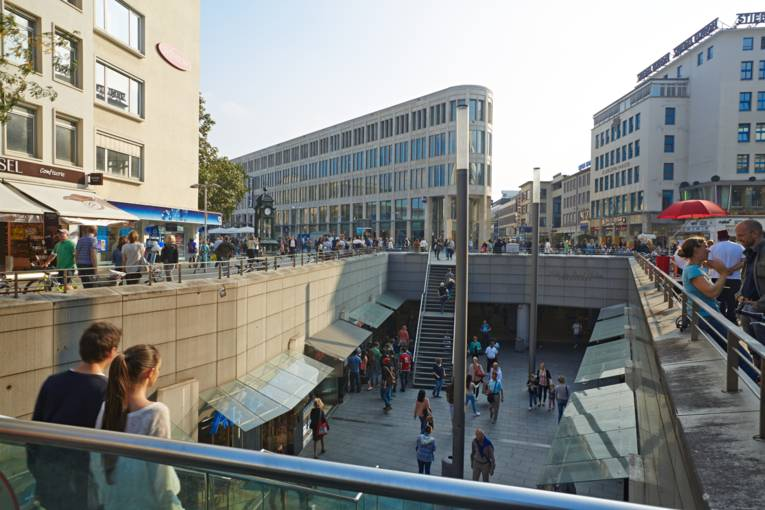
\includegraphics[width=\textwidth]{hannover-1}
		\end{column}
		\begin{column}{.45\textwidth}
			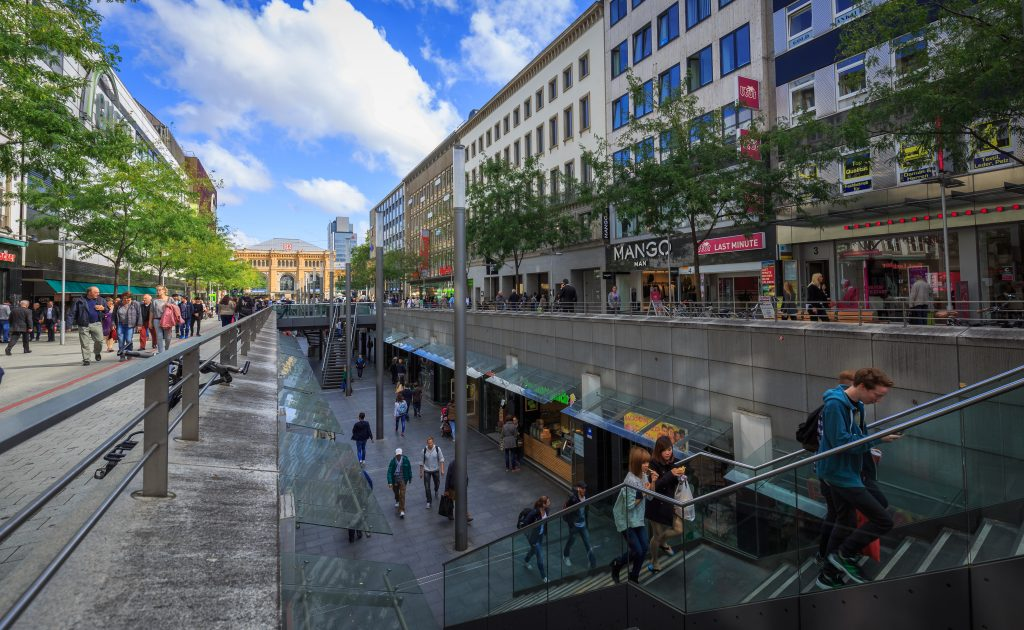
\includegraphics[width=\textwidth]{hannover-2}
		\end{column}
	\end{columns}	
	\begin{columns}
		\begin{column}{.45\textwidth}
			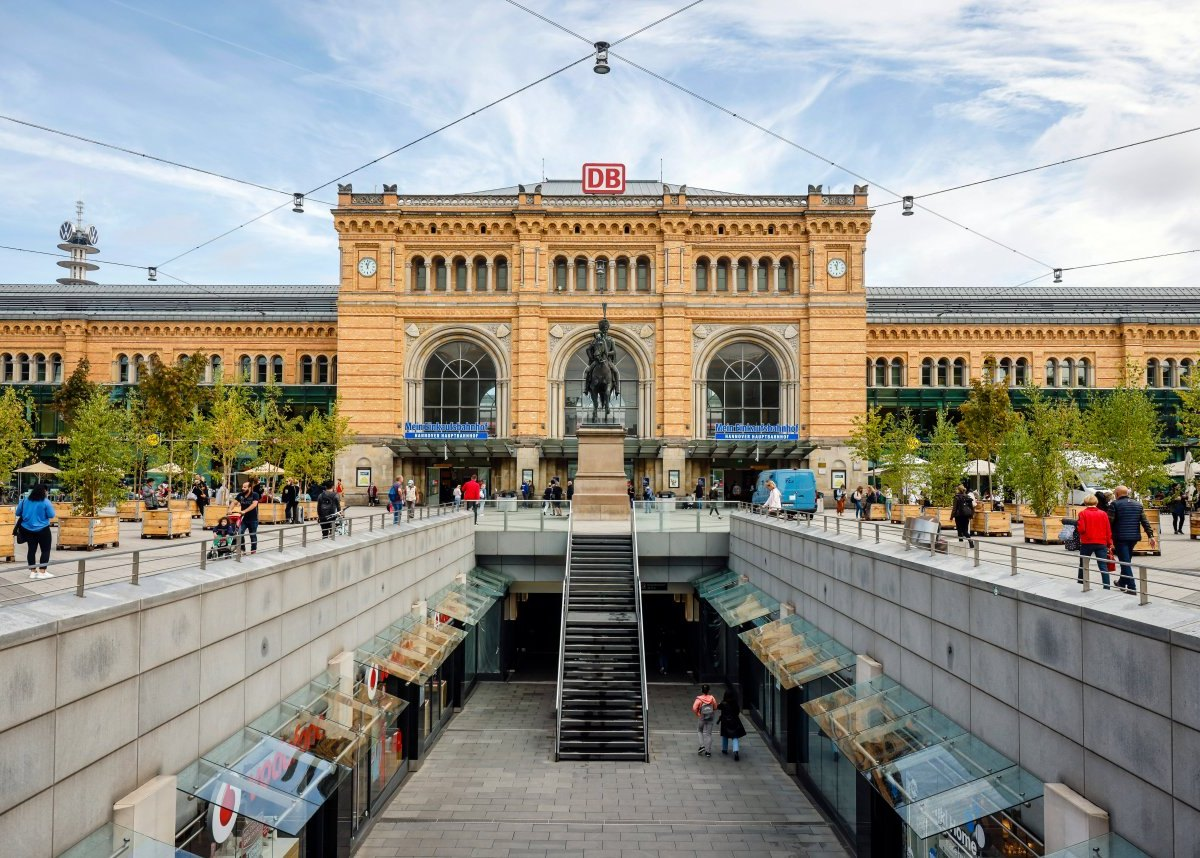
\includegraphics[width=\textwidth]{hannover-3}
		\end{column}
	\end{columns}
\end{frame}

\subsection{How are trains done in Bratislava}

\begin{frame}
	\frametitle{Stanica Bratislava predmestie???}

	\begin{columns}
		\begin{column}{.45\textwidth}
			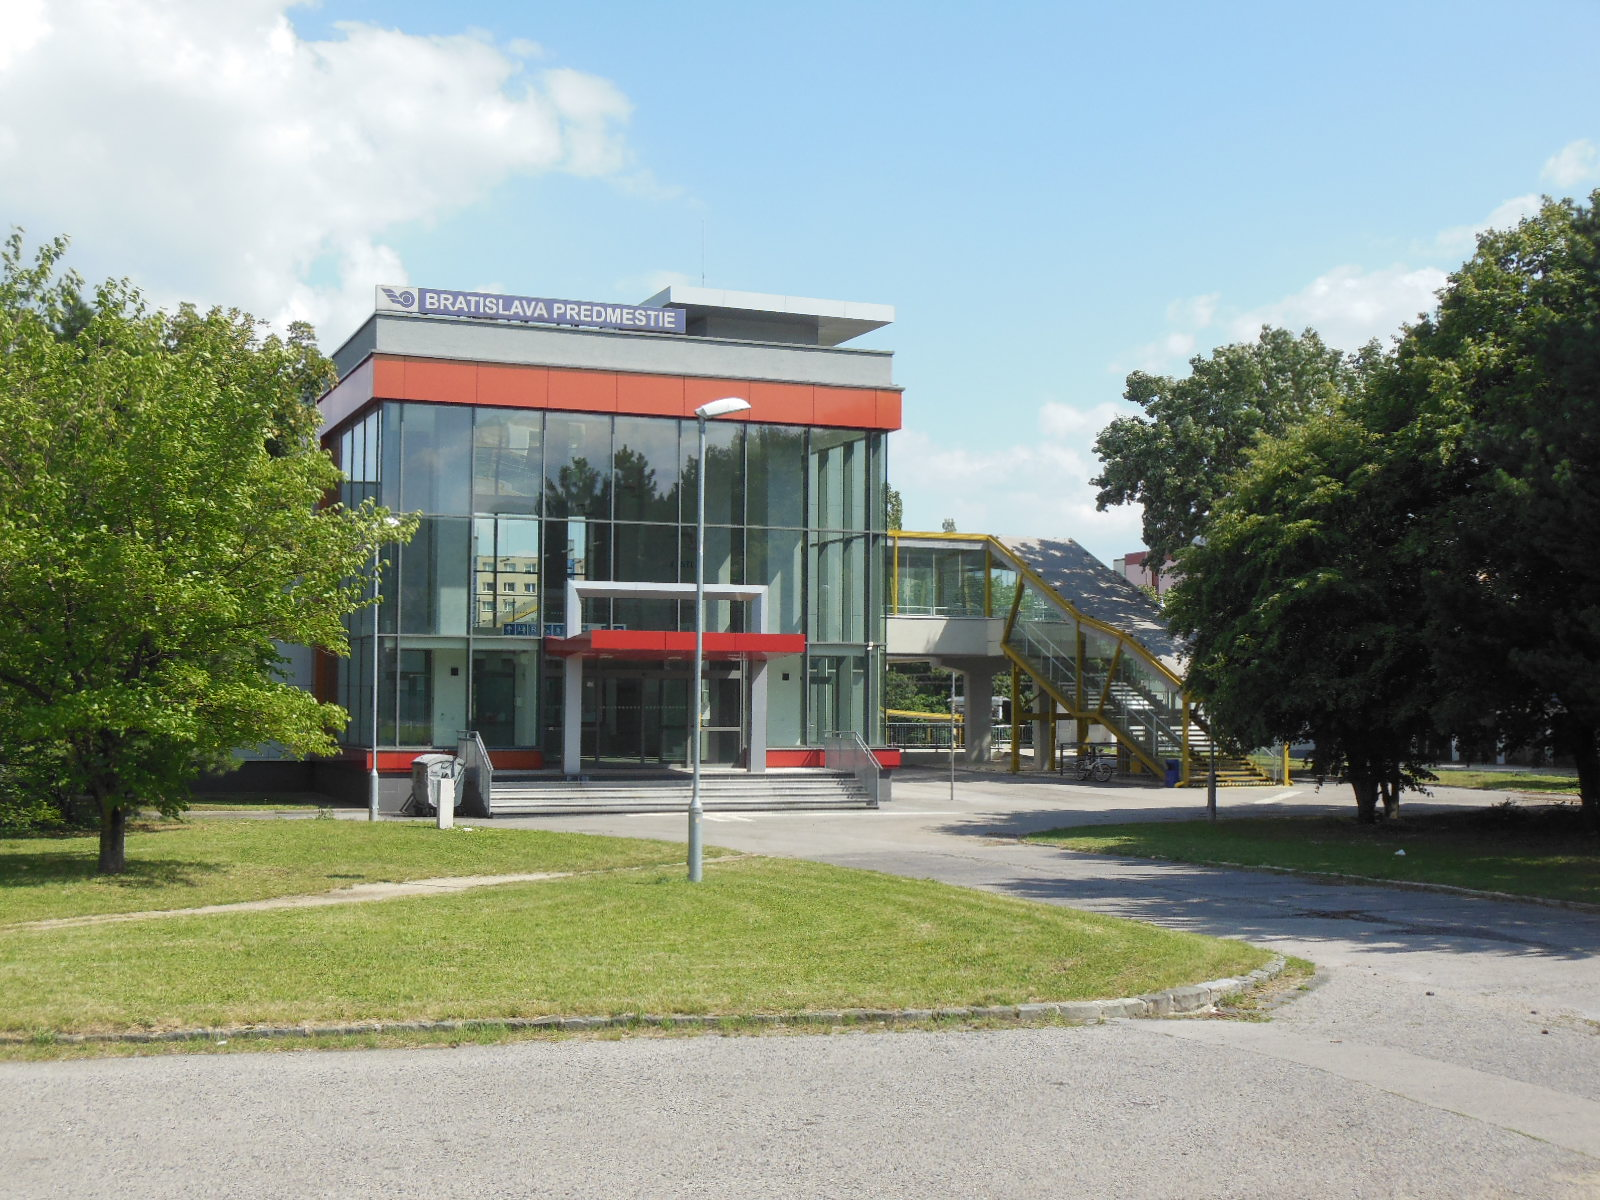
\includegraphics[width=\textwidth]{bratislava-predmestie}
		\end{column}
		\begin{column}{.45\textwidth}
			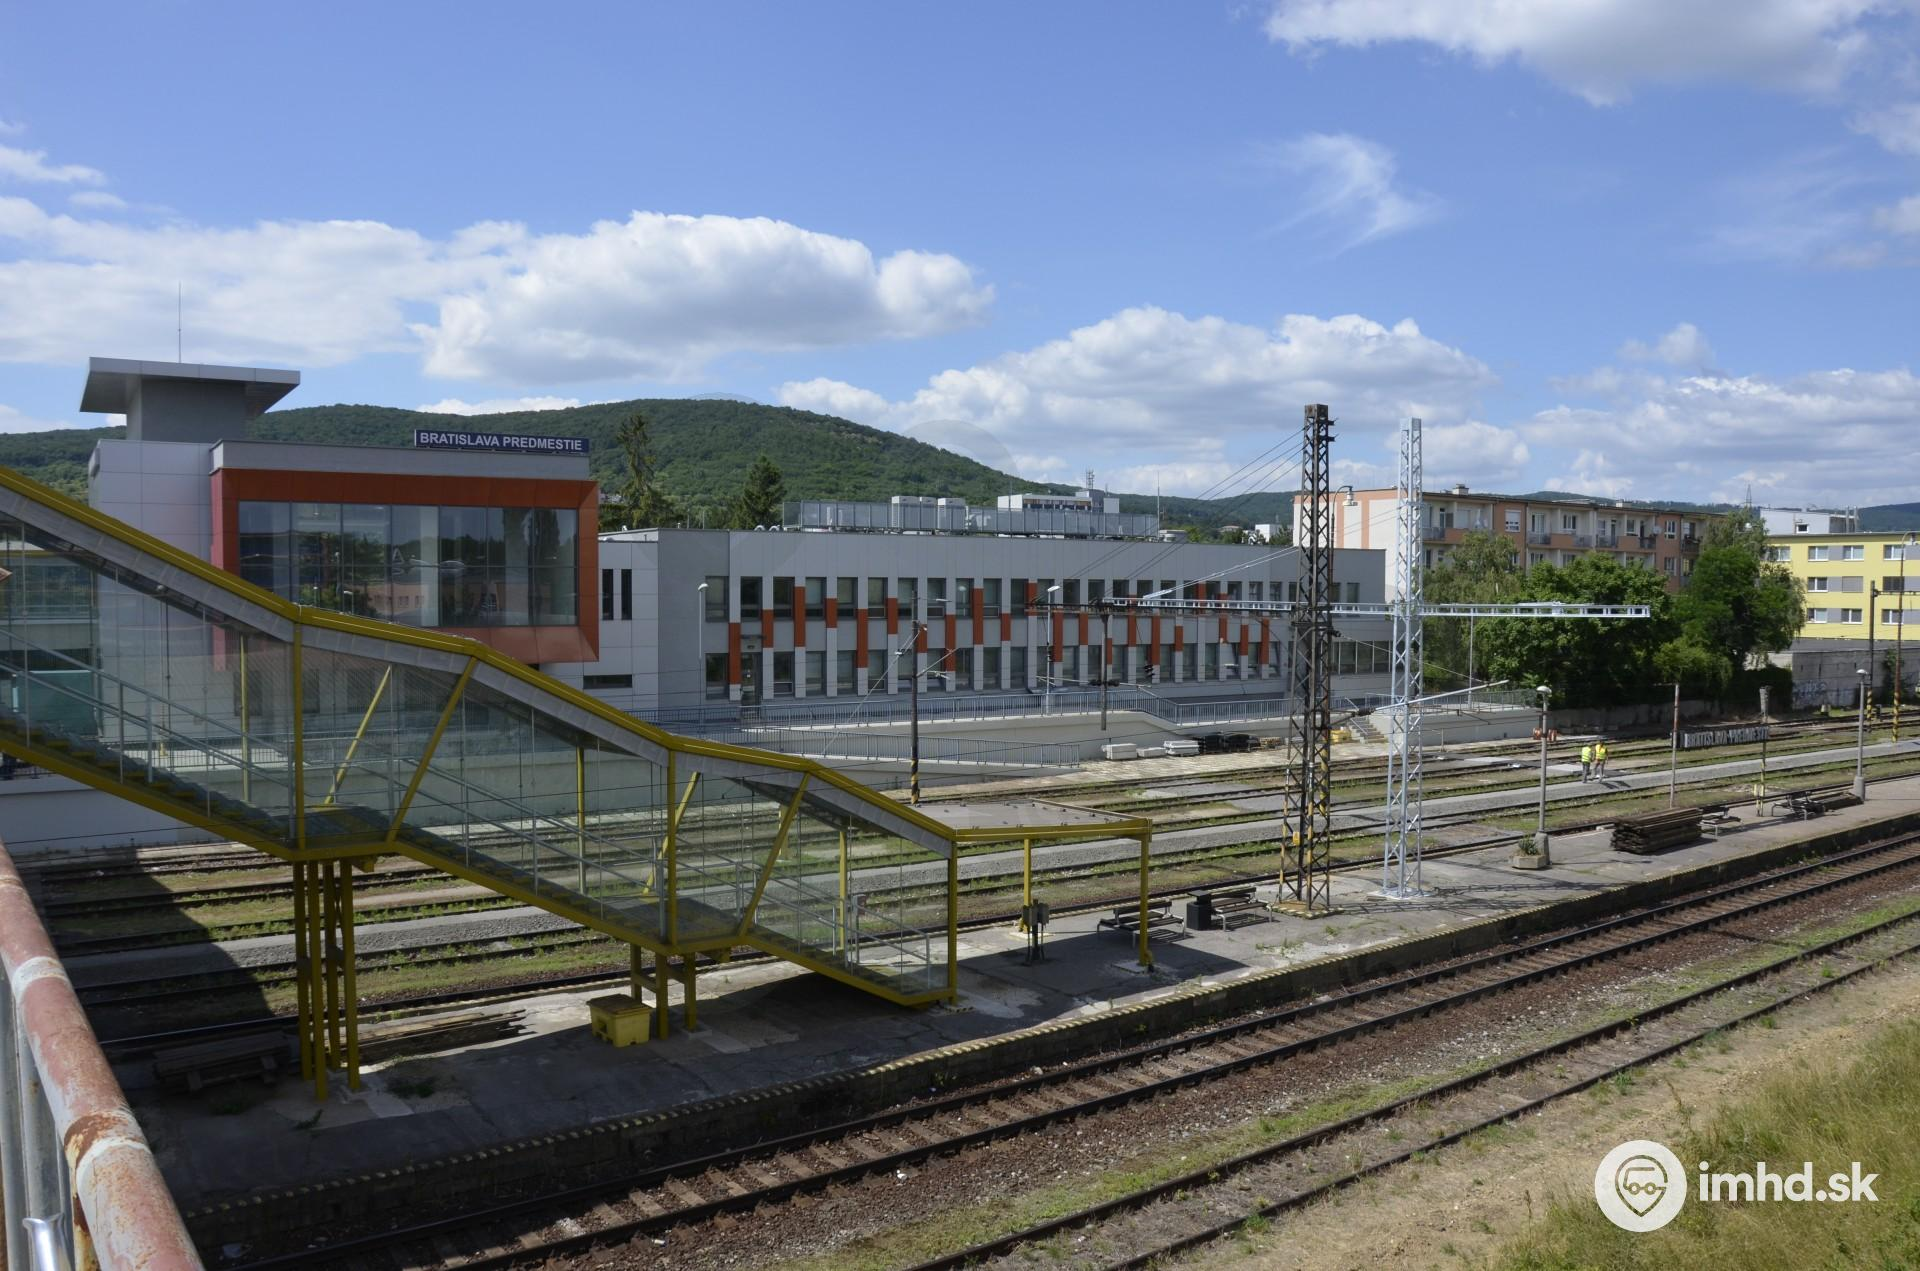
\includegraphics[width=\textwidth]{bratislava-predmestie-2}
		\end{column}
	\end{columns}	
	\begin{columns}
		\begin{column}{.45\textwidth}
			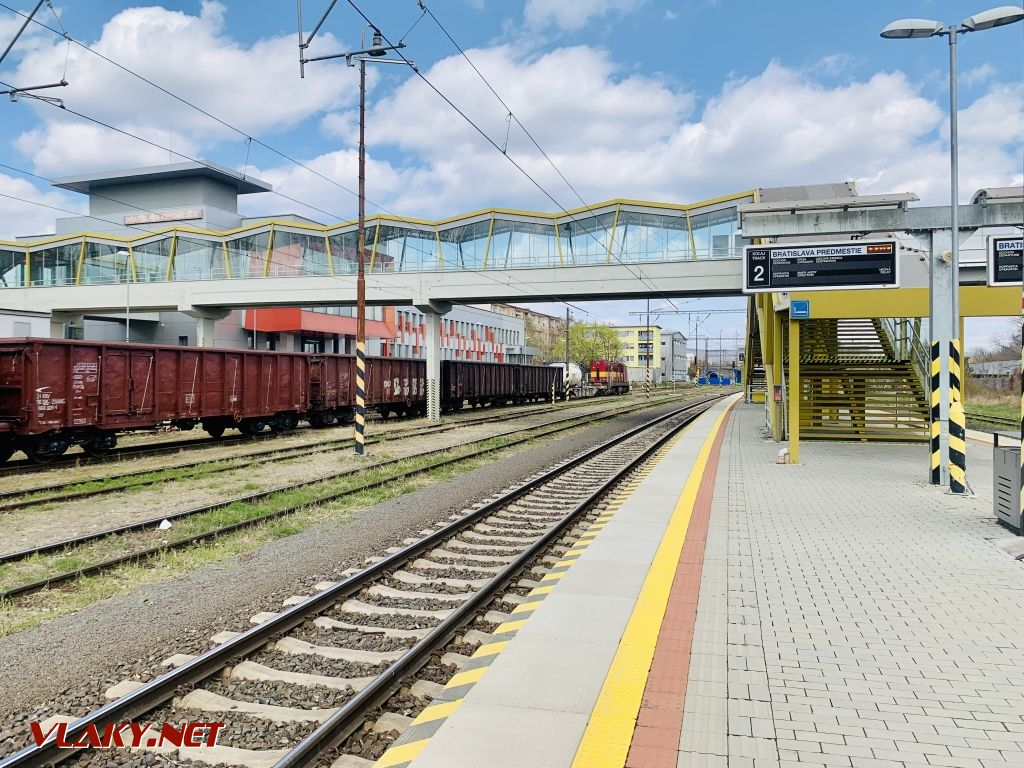
\includegraphics[width=\textwidth]{bratislava-predmestie-1}
		\end{column}
		\only<2>{
			\begin{column}{.45\textwidth}
				\begin{enumerate}
					\item 7 passanger trains daily
					\item reconstructed in 2017 for 8.9million
				\end{enumerate}
			\end{column}
		}
	\end{columns}
\end{frame}

\begin{frame}
	\frametitle{Stanica Bratislava Petžalka}

	\begin{columns}
		\begin{column}{.5\textwidth}
			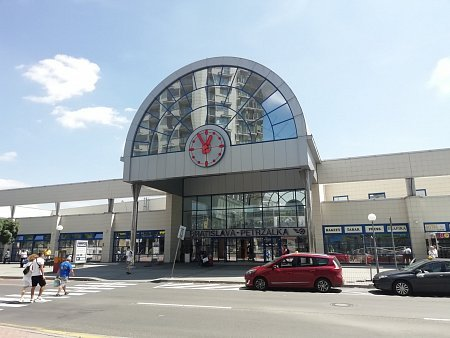
\includegraphics[width=\textwidth]{bratislava-petrzalka-2}
		\end{column}
		\begin{column}{.5\textwidth}
			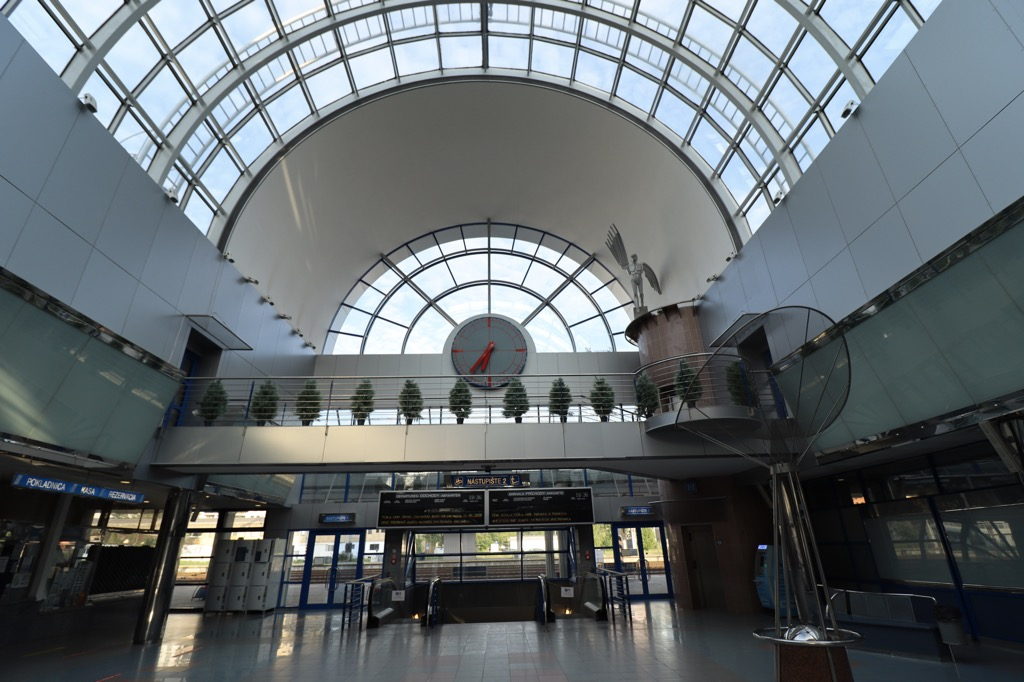
\includegraphics[width=\textwidth]{bratislava-petrzalka-4}
			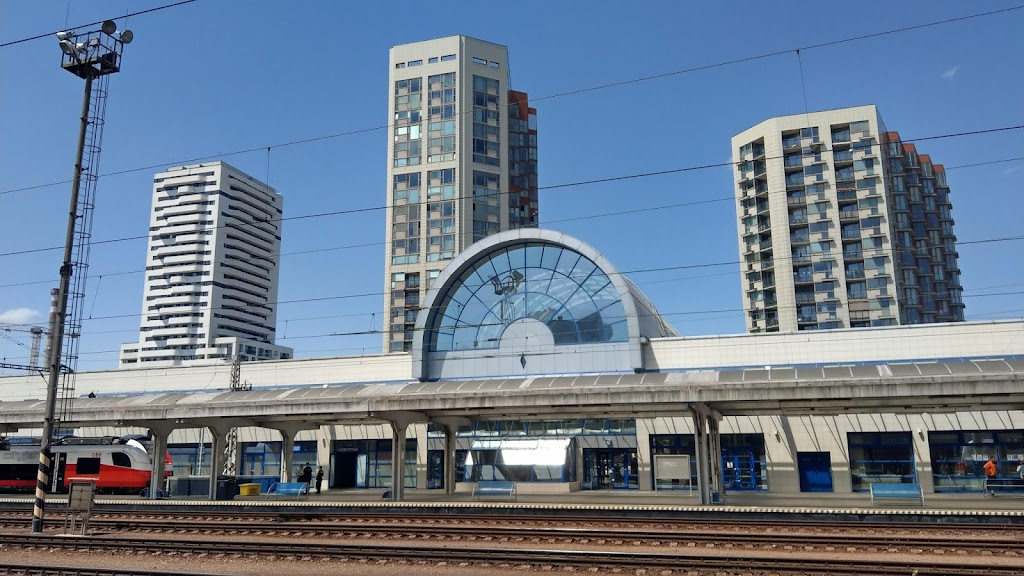
\includegraphics[width=\textwidth]{bratislava-petrzalka-3}	
		\end{column}

	\end{columns}
\end{frame}

\begin{frame}
	\frametitle{Orientácia stanice Bratislava Petžalka}

	\begin{columns}
		\begin{column}{.45\textwidth}
			
\includegraphics[width=\textwidth]{spidey-top}\\
			\only<2>{
\includegraphics[width=\textwidth]{spidey-bottom}}
		\end{column}
		\begin{column}{.45\textwidth}
			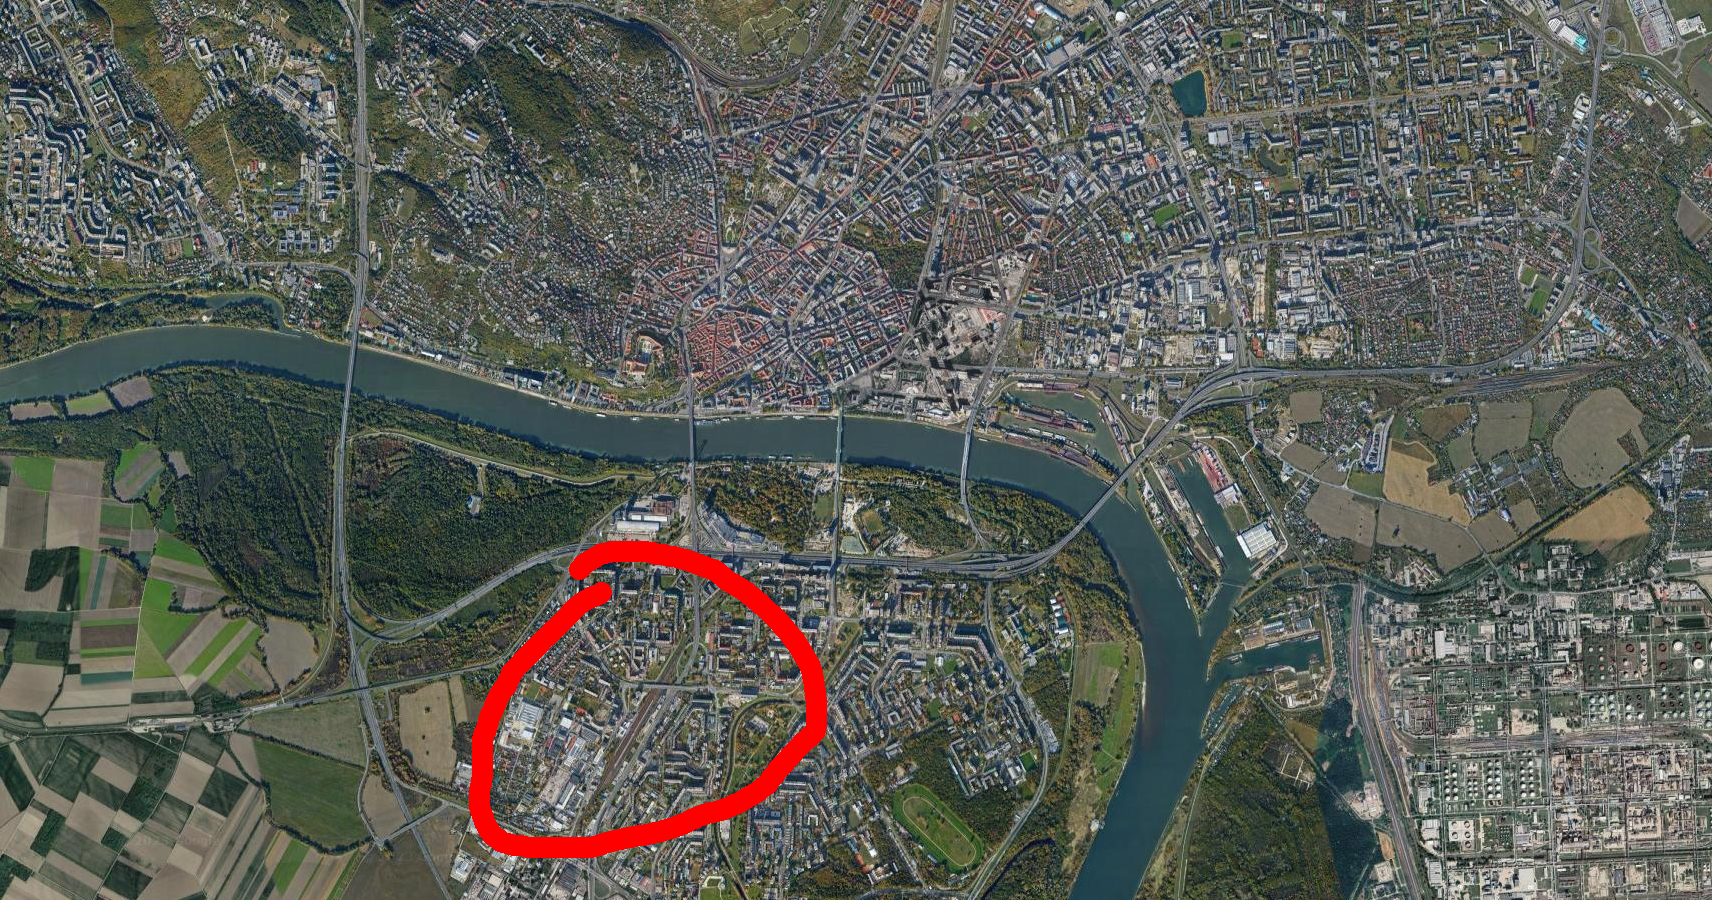
\includegraphics[width=\textwidth]{bratislava-petrzalka-topdown-1}
			\\[2em]
			\only<2>{
				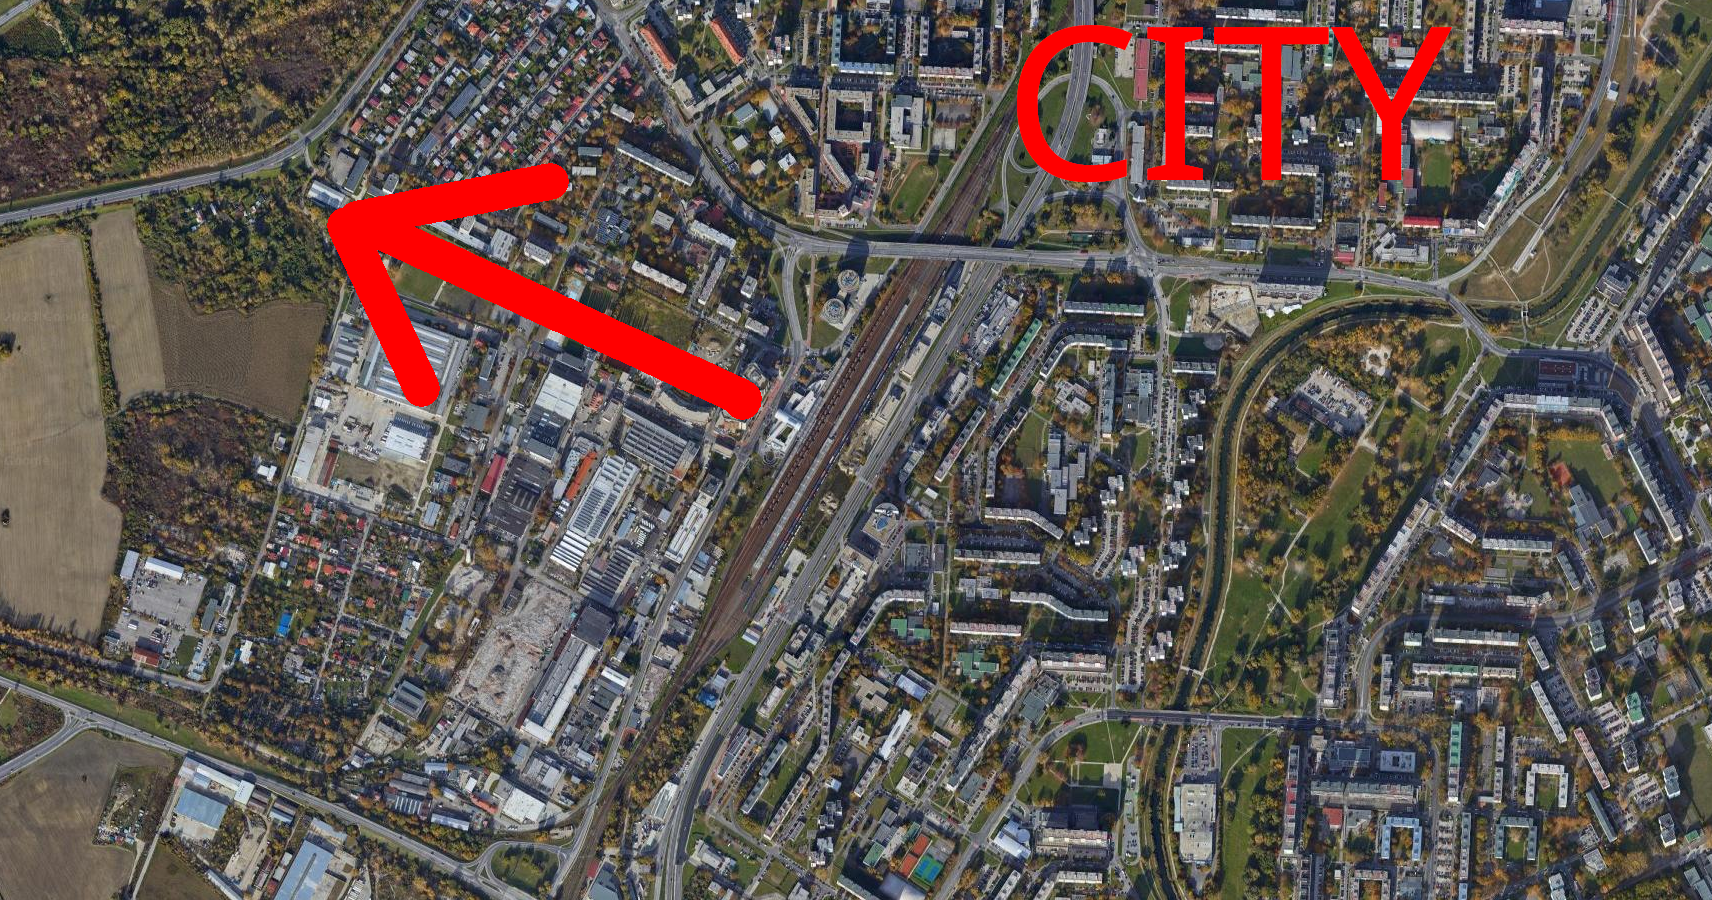
\includegraphics[width=\textwidth]{bratislava-petrzalka-topdown-2}
			}
		\end{column}
	\end{columns}
\end{frame}


\begin{frame}
	\begin{columns}
		\begin{column}{.5\textwidth}
			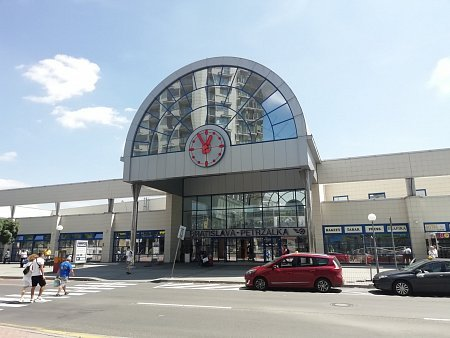
\includegraphics[width=\textwidth]{bratislava-petrzalka-2}
		\end{column}
		\begin{column}{.5\textwidth}
			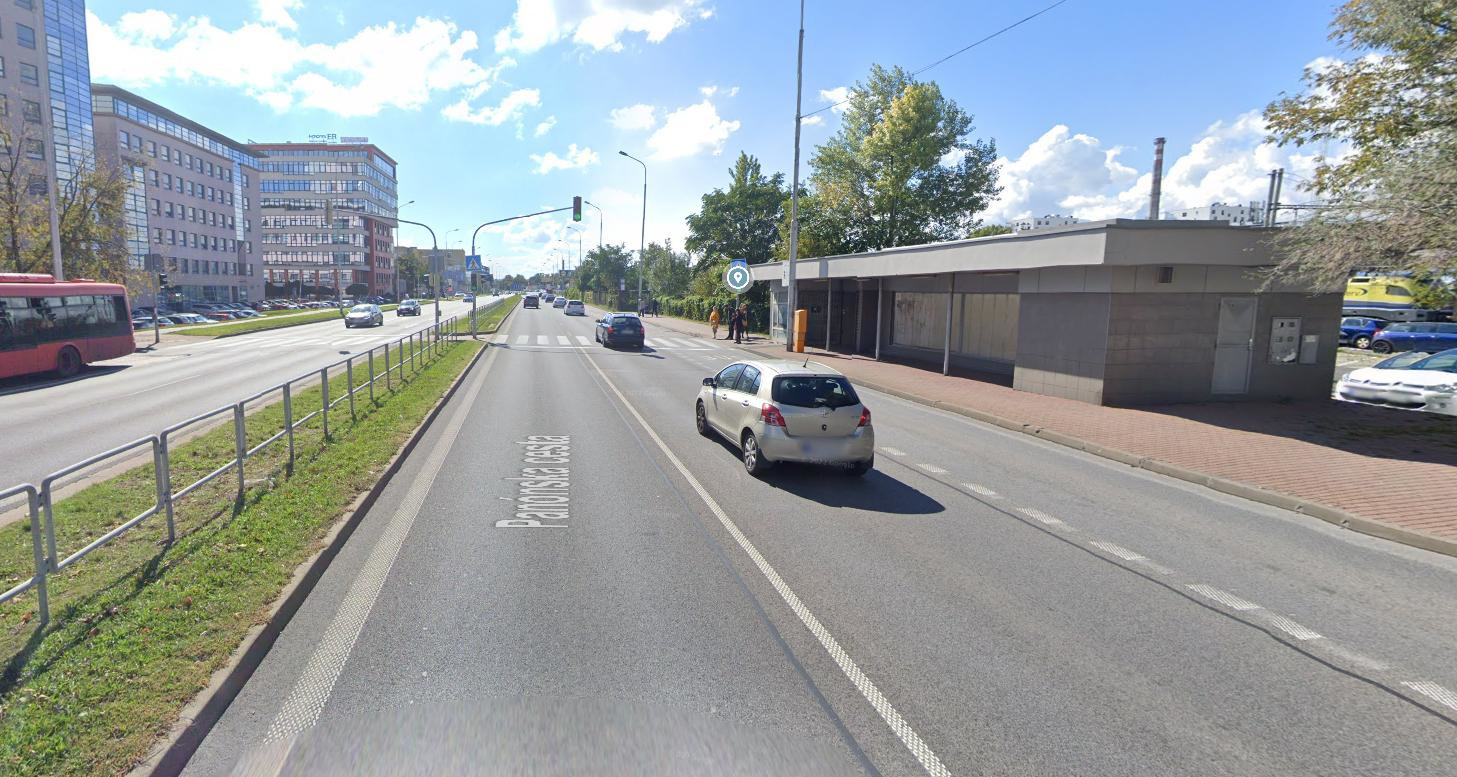
\includegraphics[width=\textwidth]{bratislava-petrzalka-1}
		\end{column}
	\end{columns}
\end{frame}


\begin{frame}
	\frametitle{Bratislava Nové Mesto}

	\centering
	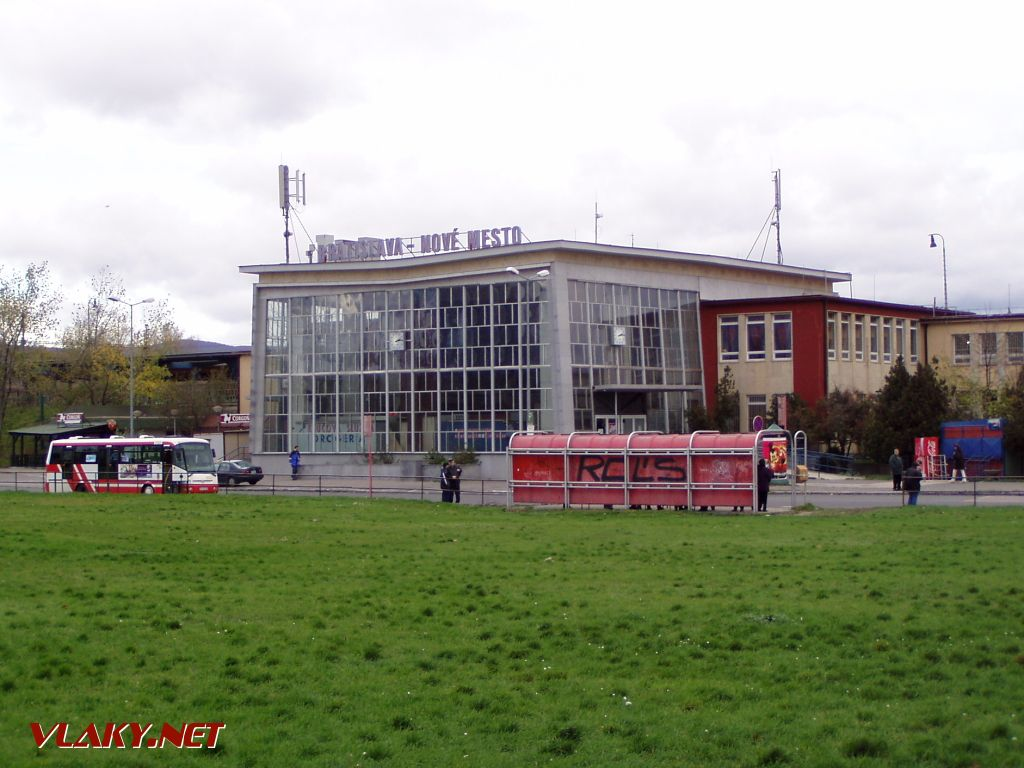
\includegraphics[width=.9\textwidth]{bratislava-nove-mesto}	
\end{frame}

\begin{frame}
	\frametitle{What's wrong}
	\begin{enumerate}
		\item Land value wasted
		\item Not central station like in other cities
		\item Unnecessary train station infrastructure
		\item Wastefull reparing
		\item Bad planning (Bratislava-Vajnory not extending the platform)
		\item Bratislava City Council has no stake or strong agreements with ŽSR
	\end{enumerate}
\end{frame}
